\chapter{基于逆向师生蒸馏（S2T）的波浪结构分类研究}

\section{问题提出}

\subsection{波浪理论量化的难点与高频噪声干扰}

承接第3章在赛马场竞争机制驱动的高维金融因子建模上的探索，本章进一步聚焦于金融时间序列中极具挑战性的拓扑形态识别——波浪结构分类。针对波浪理论与市场预测中的分类问题，本章旨在通过深度学习与多智能体协同机制，打破传统主观形态分析与现代量化交易之间的壁垒。艾略特波浪理论由Elliott于20世纪提出，其核心观点为：市场波浪运动遵循``五浪推进+三浪调整''的循环模式，且该模式在不同时间尺度上递归嵌套，呈现显著的分形特征\cite{tirea2012stock}。在实践中，该理论已被广泛用于波浪延续与反转识别、价格路径预测及风险区域划定\cite{dangelo2017effectiveness}。图~\ref{fig:placeholder}展示了艾略特波浪理论的基本结构，包括五浪推进与三浪调整的典型形态及其分形嵌套关系。

\begin{figure}[htbp]
    \centering
    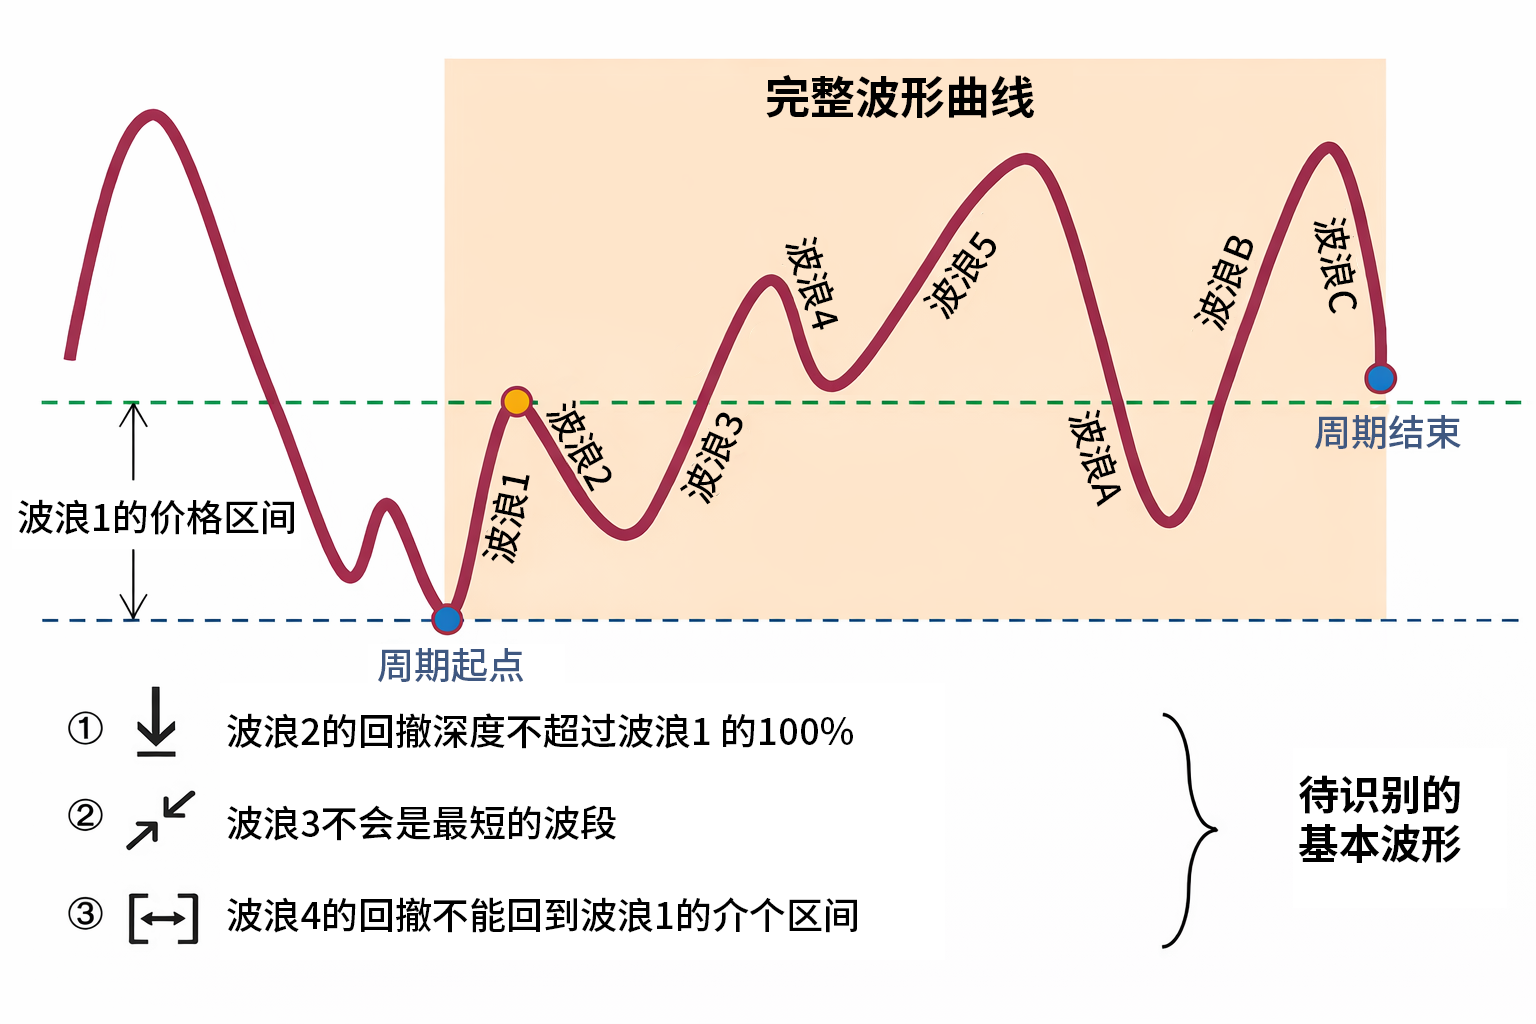
\includegraphics[width=1\linewidth]{figures/chap5/bolang.png}
    \caption{Elliott波浪理论}
    \label{fig:placeholder}
\end{figure}

然而，金融市场固有的高频噪声与结构模糊性，导致仅有部分波浪片段具备实际预测价值。在高频数据环境中，传统依赖人工划分的波浪理论面临明显瓶颈：波浪边界存在显著主观性，不同分析者之间划分容易出现不一致\cite{wawer2024large}；波浪尺度随市场波动强度动态变化，使规则驱动方法难以保持稳定性。传统艾略特波浪理论虽然在刻画市场分形特征与层级嵌套上具有深刻的直觉，但其高度的主观性与边界模糊性使其难以直接应用于高频量化交易。具体而言，波浪理论量化面临三重核心挑战：第一，波浪边界的模糊性，即同一段价格序列可能被不同分析者划分为截然不同的浪型结构，缺乏统一的判定标准；第二，多尺度嵌套的复杂性，波浪理论要求在不同时间尺度上同时识别推进浪与调整浪的递归结构，这对特征提取的层次性提出了极高要求；第三，高频噪声的干扰性，在日内或日频数据中，大量随机波动会产生伪结构信号，使模型难以区分真实的趋势转折与短暂的价格扰动。

深度学习在金融时间序列预测中展现出显著优势，LSTM网络和Transformer模型因能够捕捉长期依赖结构，被广泛应用于趋势检测、波动率预测与交易信号生成\cite{fischer2018deep,sirignano2021universal,nelson2017stock}；生成对抗网络（GAN）在合成金融序列与极端场景模拟中同样表现出独特潜力\cite{wiese2020quant,vuletic2024fin}。为了充分利用深度学习的表征能力，本章构建了生成器判别器组，将生成对抗范式引入金融序列的结构化建模中。然而，传统深度学习模型在金融结构化信号建模方面仍存在关键瓶颈：金融时间序列具有典型的非平稳性、突变性与多尺度结构，宏观趋势、局部波段与高频噪声往往交织并存，使模型难以稳定捕捉隐含的层级结构特征\cite{hamilton1989regime,Cont2001Empirical}。现有研究大多聚焦于直接预测价格或简单分类标签\cite{fischer2018deep}，忽视了金融市场价格运动本身的``结构性''，纯深度学习模型难以从高噪声序列中无监督地学习到波浪式结构化知识\cite{OZBAYOGLU2020106384}。

\subsection{传统``强教弱''蒸馏范式的局限性}

知识蒸馏（Knowledge Distillation, KD）由Hinton等人提出，其核心思想是通过教师模型向学生模型传递软标签或中间层表示，在保持模型轻量化的同时提升泛化能力\cite{hinton2015distilling}。此后，KD被扩展至多教师蒸馏、在线蒸馏与互学习等多种变体，并在图像分类、自然语言处理与时序建模等任务中得到广泛验证\cite{gou2021knowledge}。多智能体系统通过多个学习主体的协同博弈与信息共享，能够在复杂、非平稳的环境中实现更鲁棒的策略学习\cite{lee2007multiagent}。在金融领域，多智能体框架已被初步应用于投资组合优化与市场微观结构建模，但在结构化波浪分类任务中的探索仍十分有限。

然而，现有KD研究大多采用``教师到学生''的单向传递范式，忽视了学生模型对教师模型的反向校正潜力；而多智能体框架在结构化金融分类任务中的应用仍十分有限，尤其缺乏针对类别极度不平衡问题的协同训练机制。在多智能体对抗训练中，普遍存在``模式崩溃''现象：较强的模型在训练后期逐渐主导对抗过程，使弱模型难以继续学习，导致多样性下降、结构表达退化\cite{goodfellow2014generative}。常规深度学习模型在面对金融序列的强噪声与结构突变时，极易发生模式坍缩，导致对局部伪结构的过拟合。这种单向的``强教弱''机制在金融市场这种高度非平稳的环境中，往往会导致整个模型群体陷入局部的次优解，丧失对全局复杂结构的探索能力。

从信息论的角度分析，传统蒸馏中教师模型的软标签虽然包含了类间关系的丰富信息，但这种信息传递是单向且静态的。在金融时间序列的非平稳环境中，教师模型可能在某些市场状态下过度自信，其软标签反而会误导学生模型。例如，在市场剧烈波动期间，教师模型可能对某类波浪结构产生系统性偏差，而学生模型由于被强制拟合教师输出，无法通过自身探索发现更准确的结构边界。这种``强教弱''的单向机制在面对金融市场的结构突变时，缺乏必要的自我纠错能力。

\subsection{逆向师生蒸馏的必要性分析}

为解决波浪理论量化与多任务分类中的模式坍缩问题，本章在第1章提出的CDVA分形方法（裸K线数据的结构化降噪）基础上，设计了创新的逆向师生蒸馏（Student-to-Teacher Distillation, S2T）系统以解决波浪分类预测难题。与传统``强教师指导弱学生''的单向蒸馏不同，S2T机制引入了``反向蒸馏机制''：当学生智能体在特定复杂结构上实现阶段性超越时，使教师模型在训练中参考学生模型学习到的新分布特征。通过逆向师生蒸馏（S2T）实现弱模型向强模型的反向校正，这种由弱模型向强模型提供补充约束的训练机制，有助于缓解强模型对局部高频噪声的过拟合问题。

本章的核心问题在于：如何将主观的波浪形态转化为可严格量化的监督学习任务，并通过多智能体协同克服类别极度不平衡带来的决策边界坍缩？为此，本章将结合VA/CD分形定义，详细阐述CDVA分形事件的数学定义，以及S2T机制在多分类预测网络中的协同训练流程。同时，结合``带鱼短鱼''机制对趋势惯性进行量化界定，验证该双向纠偏机制在方法改进中发挥的重要作用。在不同任务下验证逆向师生蒸馏系统（S2T-Wave）的性能优势，本章提出的CDVA结构标签体系与基于多模型协同的S2T框架，正是旨在弥补上述不足，将波浪理论的分形结构先验与深度学习的端到端优化能力有机融合。图\ref{fig:S2T-arch}展示了基于S2T的波浪分类预测整体组织架构，图\ref{fig:S2T-task}展示了对应的多任务预测任务设置。

\begin{figure}[htbp]
    \centering
    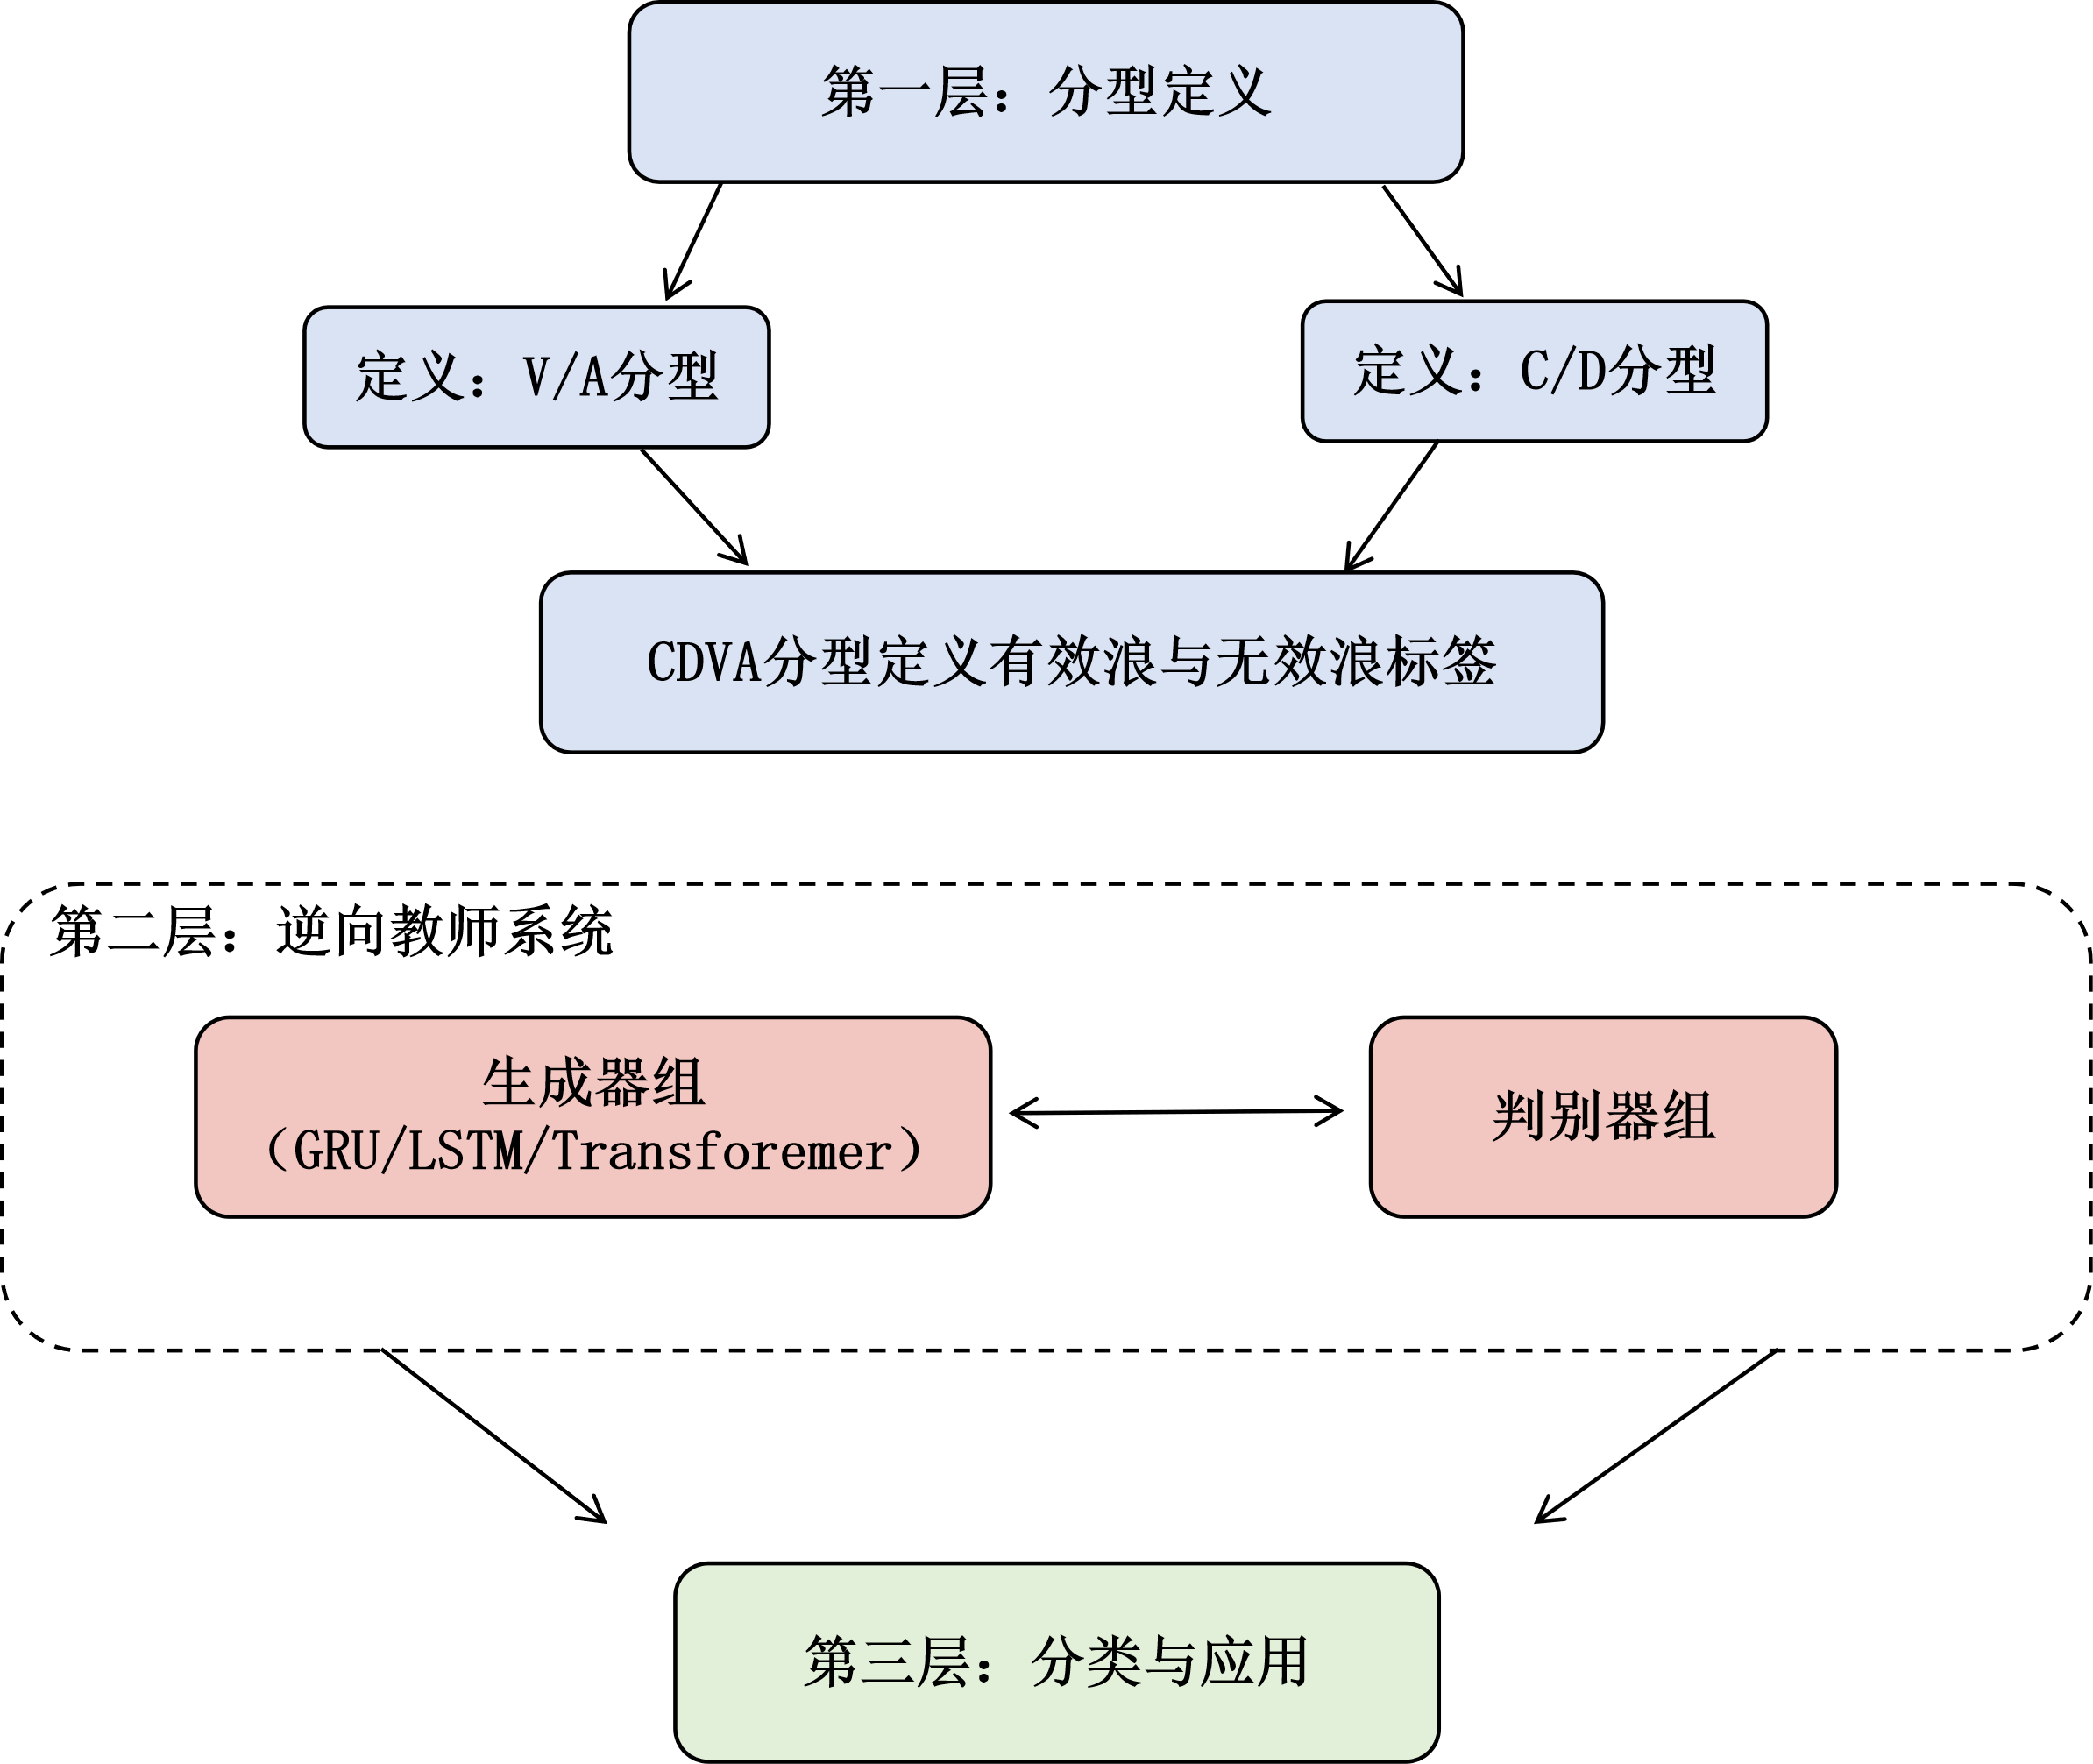
\includegraphics[width=0.8\textwidth]{figures/chap5/波浪架构.png}
    \caption{基于S2T的波浪分类预测组织架构}
    \label{fig:S2T-arch}
\end{figure}

\begin{figure}[htbp]
    \centering
    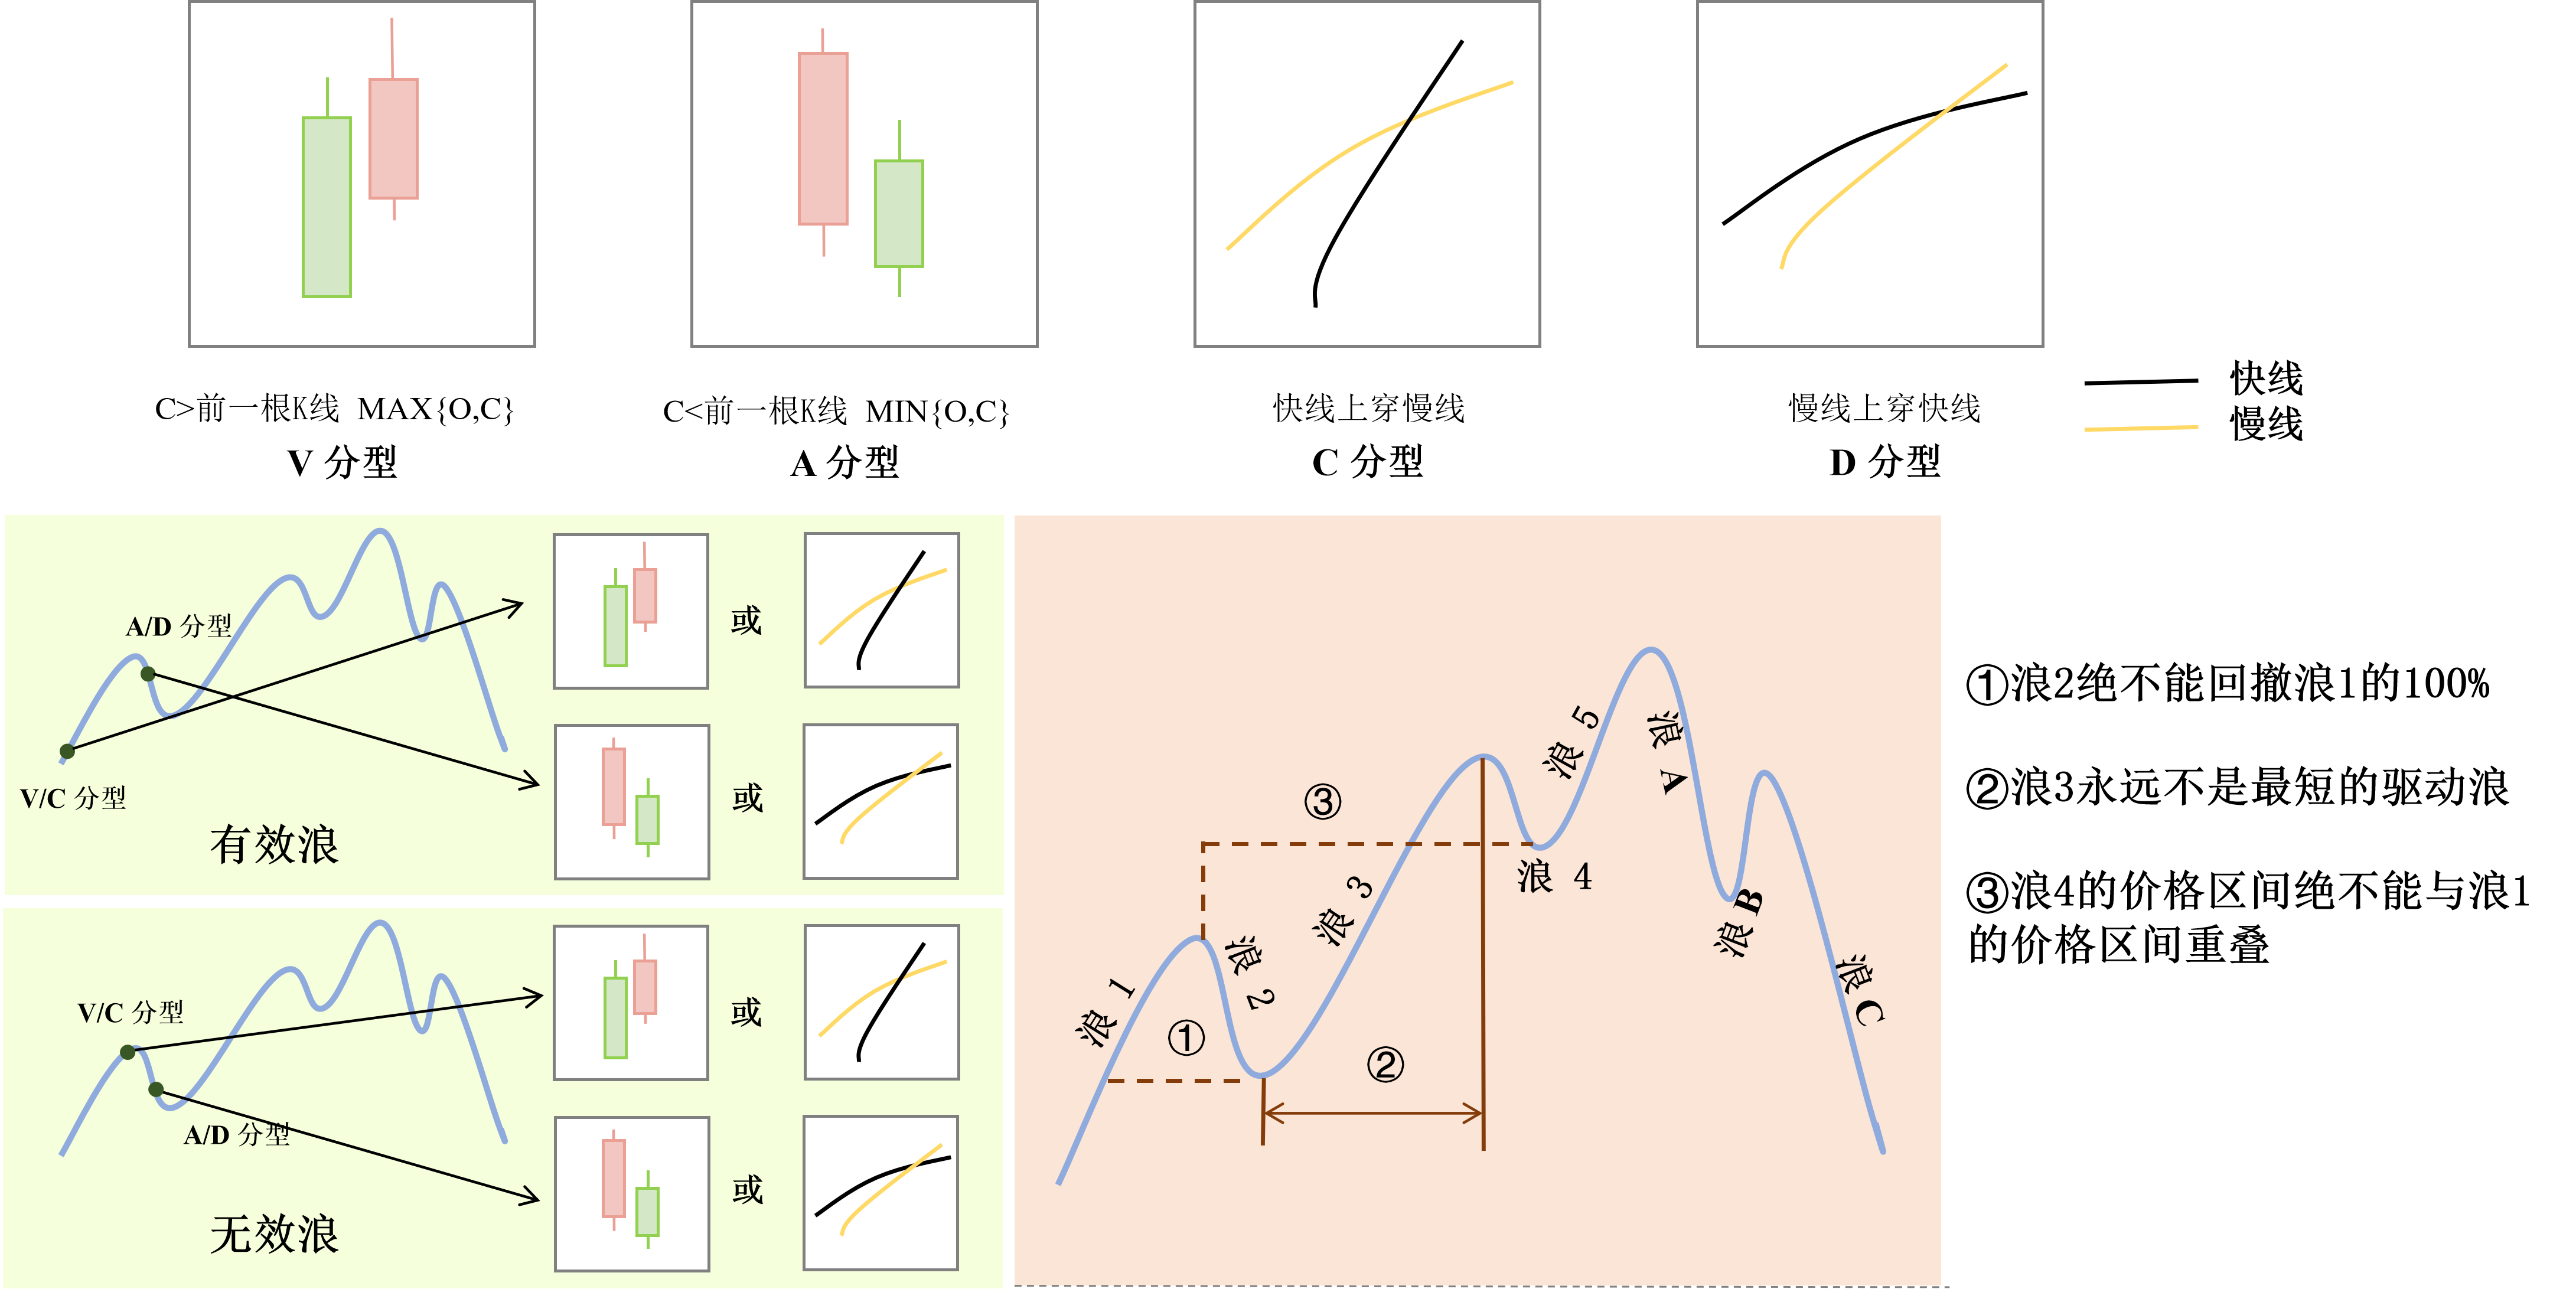
\includegraphics[width=0.8\textwidth]{figures/chap5/波浪任务.png}
    \caption{基于S2T的波浪分类预测任务}
    \label{fig:S2T-task}
\end{figure}

\section{CDVA分形方法与波浪量化重构}

\subsection{C/D/V/A四类分形事件的数学定义}

``裸K线交易法''（Naked K-Line Trading）强调在交易图表中剔除均线、MACD、布林带等衍生指标，仅依据原始K线（蜡烛图）的形态、组合排列及关键支撑阻力位分析市场微观结构。这类方法直观、贴近交易实践，但其判断过程很大程度上依赖视觉经验，长期缺乏可重复的数学边界。与之相对，传统深度学习模型虽然能够处理连续价格序列，却往往把价格变化压缩为浮点数张量，弱化了K线之间最基本的拓扑排列关系，使结构判定与模型输出之间缺乏直接对应。

基于这一问题，本章提出 CDVA 分形方法。其中，V（向上突破）与 A（向下跌破）分型对应于相邻K线之间最基础的突破与跌破结构。通过对前一周期实体边界与当前收盘价之间的关系进行明确刻画，原本依赖经验识别的K线排列被转化为可重复的二元事件标签。这样处理的目的，不是简单增加一组技术指标，而是为后续模型训练提供结构化输入，并使输出结果仍然能够回到原始K线图上解释。换言之，CDVA 试图打通裸 K 线经验与深度模型之间的语义壁垒，使模型输出能够回到原始图表上做到“所见即所得”式的解释。

为了构建可用于深度模型训练的结构化波浪标签体系，本章基于动量类指标与K线结构行为，设计了四类分形事件：C（上穿）、D（下穿）、V（向上突破）、A（向下跌破）。相比传统波浪结构定义，该体系更易量化、边界明确、对噪声敏感度低，能够在大规模时序数据上实现稳定标注。四类分形事件的设计遵循两个核心原则：其一，C与D基于动量指标的方向切换，捕捉趋势的宏观转折信号；其二，V与A基于K线实体的价格突破，捕捉微观层面的结构性波动。这种宏观与微观相结合的标签设计，使得模型能够在多个时间尺度上同时学习波浪结构特征。

在构建C（上穿）与D（下穿）两类方向性切换分形时，本章引入了指数平滑异同移动平均线（MACD）。MACD由快速与慢速两条指数加权移动平均线（EMA）构成，二者之差定义为动量线（DIF）：

\begin{equation}
\mathrm{DIF}_t = \operatorname{EMA}_{\text{fast}}(P_t) - \operatorname{EMA}_{\text{slow}}(P_t),
\end{equation}

其中$P_t$为时刻t的收盘价。DIF的指数移动平均为信号线（DEA），二者之差称为MACD柱状线：

\begin{equation} \mathrm{DEA}_t = \operatorname{EMA}_{\text{signal}}(\mathrm{DIF}_t) \label{eq:dea} \end{equation}

\begin{equation} \mathrm{MACD}_t = 2 \times (\mathrm{DIF}_t - \mathrm{DEA}_t) \label{eq:macd} \end{equation}

本章将MACD重新解释为``分形结构触发器''：当DIF由下向上穿越DEA时记为C（金叉）；当DIF由上向下穿越DEA时记为D（死叉）。相比传统手工波浪划分，这种基于MACD的结构事件更具可量化性、鲁棒性与可重复性。需要指出的是，MACD本身作为滞后指标，其信号触发时间通常晚于价格的实际转折点，这一特性在后续的``带鱼短鱼''机制中将被进一步讨论与补偿。

在方向性切换分形的基础上，本章进一步定义基于K线实体突破的结构性波动事件（V/A）。给定上一周期实体上沿与下沿：

\begin{equation}
U_{t-1} = \max(\mathrm{open}_{t-1},\, \mathrm{close}_{t-1}),
\qquad
L_{t-1} = \min(\mathrm{open}_{t-1},\, \mathrm{close}_{t-1}),
\end{equation}

则当前周期的V/A信号定义为：

\begin{equation}
V_t = \mathbb{I}(\mathrm{close}_t > U_{t-1}),
\qquad
A_t = \mathbb{I}(\mathrm{close}_t < L_{t-1}).
\end{equation}

V描述价格向上穿越前实体上沿的``结构性突破''，常对应趋势波段的延续；A描述价格向下跌破前实体下沿的``结构性回落''，常预示反转或加速回撤。V/A的定义基于严格的价格边界，对噪声不敏感，可在高频/日频数据上稳定复现。与C/D分形相比，V/A分形具有更高的时间分辨率，能够在趋势内部捕捉到更细粒度的结构变化，为模型提供了互补的多尺度结构信息。

基于上述定义，CDVA 标签体系将波浪结构识别转化为可重复的监督信号，并为后续 4.3 节的模型构建与 4.4 节的实验比较提供统一的结构标签基础。

\subsection{结构化降噪与艾略特波浪理论量化重构}

在 CDVA 分形标签体系的基础上，本章进一步引入``带鱼短鱼''机制，用于回答另一个更接近交易实践的问题：结构信号出现之后，是否真的走成了一段可持续的有效趋势。趋势跟随策略通常难以吃到趋势启动初期的``鱼头''，也很难保留反转阶段的``鱼尾''，真正决定策略盈亏的，往往是中段那一段是否足够完整、是否具有延续性。基于这一考虑，本文将持续时间较长、终点价格优于起点价格的有效波段记为``带鱼''（Long Fish），将信号触发后较快反转、未形成有效收益的失败波段记为``短鱼''（Short Fish）。其核心不是评价信号出现得是否“漂亮”，而是考察信号触发后的价格演化是否真正兑现了趋势承诺。

这一划分为艾略特波浪理论中``有效浪''与``无效浪''的区分提供了可计算形式。将其纳入逆向师生蒸馏（S2T）系统后，模型学习的对象不再只是局部结构是否出现，还包括该结构能否延续为有效趋势，从而为后续分类任务提供更稳定的监督信号。以 MACD 金叉位置为波段起点 $t_s$，下一次反向信号（死叉）位置为波段终点 $t_e$，并以终点价格是否优于起点价格作为趋势有效性的判定准则：

\begin{equation}
\text{Label}_{[t_s, t_e]} =
\begin{cases}
\text{Long Fish}, & \text{if } P_{t_e} > P_{t_s} \quad \text{（看涨波段）} \\
\text{Short Fish}, & \text{if } P_{t_e} \leq P_{t_s} \quad \text{（看涨波段）}
\end{cases}
\end{equation}

对称地，在下跌趋势中：

\begin{equation}
\text{Label}_{[t_s, t_e]} =
\begin{cases}
\text{Long Fish}, & \text{if } P_{t_e} < P_{t_s} \quad \text{（看跌波段）} \\
\text{Short Fish}, & \text{if } P_{t_e} \geq P_{t_s} \quad \text{（看跌波段）}
\end{cases}
\end{equation}

这一机制可视为对 CDVA 分形划分的应用扩展。CDVA 负责识别结构事件何时出现，``带鱼短鱼''则进一步回答这些结构是否真正转化为可持续的收益结构。若只看交叉或突破本身，模型容易学到大量假突破；而加入带鱼判定后，模型学习的对象同时包含“结构出现”与“结构是否走成”，从而更接近交易者真正关心的问题。

这一机制将``波段是否成功''转化为可观测、可训练的二元标签，解决了传统方法只能识别结构、不具备有效性验证机制的问题。从统计学角度来看，在本章所使用的15种期货品种的日频数据中，``短鱼''波段的数量通常占总波段数的60%至75%，呈现出典型的类别不平衡特征。这一分布特点进一步凸显了在模型训练中采用Focal Loss等不平衡处理策略的必要性。

从这一意义上看，本章最终形成的是一个“结构—有效性”两级标注框架：前层由 C/D/V/A 分形描述市场中的结构事件，后层由带鱼短鱼判定这些结构是否具备趋势持续性。这样处理既保留了波浪理论对结构的关注，也把无效信号过滤纳入可监督学习流程，为后续 S2T 机制提供了更稳固的标签基础。

\subsection{状态空间构建与特征提取优化}

在明确了C、D、V、A四类分形事件的边界与触发条件后，本章将波浪结构识别转化为一个基于多变量时间序列的多任务学习问题。给定长度为T的金融时间序列$X = \{x_1, x_2, \dots, x_T\}$，其中$x_t \in \mathbb{R}^d$表示t时刻的d维特征向量，时间窗口大小为W，模型在t时刻的输入为$X_{t-W+1:t} \in \mathbb{R}^{W \times d}$。本章的任务目标是学习一个深度映射函数$f_\theta$，预测目标空间包含两部分：结构分类标签$y_t$ = ($y^C_t, y^D_t, y^V_t, y^A_t$)属于$\{0, 1\}^4$，其中$y^k_t = 1$表示第k类分形事件发生；结构持续时间$l_t$ = ($l^C_t, l^D_t, l^V_t, l^A_t$)$\in \mathbb{R}^4$，表示对应分形结构从触发到结束的时间跨度。整体任务形式化为：

\begin{equation}
    (\hat{\mathbf{y}}_t, \hat{\mathbf{l}}_t) = f_\theta(\mathbf{X}_{t-W+1:t})
\end{equation}

其中$\hat{y}_t \in [0, 1]^4$为各分形事件发生的预测概率，$\hat{l}_t$为预测的持续时间。通过这一形式化定义，传统波浪理论中主观、模糊的``形态识别''过程被严格转化为可端到端优化的多标签分类与回归联合预测任务。

为验证基于CDVA分形模式的趋势识别方法及多智能体结构学习框架的有效性，本章选取中国商品期货市场具有代表性的15种主要期货品种作为研究对象，覆盖金属、农产品、能源化工及软商品等多个行业板块。所有数据均来自公开市场的日度行情，包含开盘价、最高价、最低价和收盘价（OHLC）等基础价格字段。本章进一步从OHLC序列中构造短周期与长周期EMA（5EMA与120EMA）、价格变化率、实体宽度、上下影线比例等派生指标。在数据预处理阶段，首先剔除所有节假日与停牌日，对缺失数据点采用前向填充方式补全，并通过滑动窗口方式对部分派生特征进行平滑处理。CDVA结构标签基于本章提出的规则系统自动完成，最终形成的输入特征包含原始价格、技术指标、一阶变化率及多尺度结构信息。

在特征工程层面，本章对输入特征进行了系统化的层次设计。第一层为基础价格特征，包括开盘价、最高价、最低价、收盘价四个原始字段；第二层为趋势敏感特征，包括5日EMA与120日EMA及其差值，用于捕捉短期与长期趋势的方向与强度；第三层为动量特征，包括MACD的DIF线、DEA线与柱状线，以及价格的一阶变化率；第四层为K线结构特征，包括实体宽度（收盘价与开盘价之差的绝对值）、上影线长度、下影线长度及其比例关系。通过这种多层次的特征构建，模型能够同时获取价格的绝对水平、相对变化趋势、动量状态与微观结构信息，为后续的多任务学习提供了丰富的输入表示。

\section{逆向师生蒸馏（S2T）系统设计}

\subsection{S2T机制的核心逻辑与``失败经验''传递}

本章构建了由多生成器（预测网络）与多判别器（结构校验网络）组成的多智能体框架。生成器组由GRU、LSTM与Transformer三类异质网络构成，以实现``局部短期记忆-全局长程依赖''的特征互补。Transformer生成器采用4层编码器结构，多头注意力机制的头数设为8，隐藏层维度为256；GRU与LSTM生成器均采用双层堆叠结构，隐藏层维度设为128。判别器组由多层感知机（MLP）与对应时序网络构成。模型输入包括OHLC基础价格序列，并辅以多尺度趋势敏感指标（5日EMA、120日EMA）以及MACD，同时包含各特征的一阶变化率，使生成器能够在``绝对水平-相对变化''两个维度中捕捉波段的结构转折行为。

选择GRU、LSTM与Transformer三种异质架构作为生成器组的设计考量在于：GRU具有较少的参数量和更快的收敛速度，适合捕捉短期局部模式；LSTM通过门控机制能够有效保留长期依赖信息，对中等时间跨度的结构特征具有优势；Transformer基于自注意力机制，能够在全局范围内建模任意位置之间的依赖关系，尤其擅长捕捉长程结构模式。三种架构的异质性确保了生成器组在特征空间中的探索多样性，为后续的蒸馏机制提供了差异化的知识来源。

为缓解模式崩溃问题，本章提出S2T，其本质是一种``双向知识流动机制''，构建正向蒸馏与反向蒸馏的对偶关系：正向蒸馏负责``收敛驱动（Exploitation）''，引导群体向当前最优解靠拢；反向蒸馏负责``发散约束（Diversity Control）''，强制强模型兼顾弱模型所保留的全局拓扑特征，防止群体同质化。

对于任意输入序列X，生成器G的输出包含四个结构分类任务（C/D/V/A）的logits输出$p_t$ = $G(X)^{(logit,t)}$，以及趋势持续时间预测$\hat{l}_t$ = $G(X)^{(len,t)}$。判别器D对输入同时输出判别logits $z = D(\cdot)^{(logit)}$与中间特征$f = D(\cdot)^{(feat)}$，分别用于对抗训练与特征蒸馏。

多任务监督损失：由于金融市场中趋势转折属于典型的低频稀疏事件，本章选择Focal Loss以动态增加少数类困难样本的梯度权重，缓解类别不平衡问题；在持续时间回归任务中采用均方误差（MSE）：

\begin{equation}
L_{\text{supervised}}
=
\sum_{t\in\{c,d,v,a\}}
\left(
\lambda_{\text{cls}}\,
\mathrm{Focal}(p_t, y_t)
+
\lambda_{\text{len}}\,
\|\hat{l}_t - l_t\|^2
\right).
\end{equation}

对抗损失：每个生成器利用组内最优判别器提供的对抗信号，使其输出的结构模式更加贴近真实数据分布：

\begin{equation}
L_{\text{adv}}
=
-\lambda_{\text{adv}}\,\mathbb{E}\,[\log D(G(X))].
\end{equation}

正向蒸馏（Teacher-to-Student）：通过验证集评分选出每组内的最优成员作为``教师模型''，教师通过带温度参数的KL散度将结构类别的分布模式传递给表现较弱的成员，同时通过MSE对趋势持续时间预测进行对齐：

\begin{equation}
L_{\text{T2S}}
=
\sum_{t}
\lambda_{\text{distill}}
\cdot
\mathrm{KL}\!
\left(
\frac{p^{(s)}_t}{\tau}
\,\Big\|\,
\frac{p^{(t)}_t}{\tau}
\right)
+
\lambda_{\text{distill}}
\cdot
\|\hat{l}^{(s)}_t - \hat{l}^{(t)}_t\|^2,
\end{equation}

其中$p^{(s)}_t$、$p^{(t)}_t$分别为学生与教师在任务$t$的输出；$\tau$为温度系数。温度参数$\tau$的引入使得教师模型的软标签分布更加平滑，从而传递更丰富的类间关系信息。在本章的实验中，$\tau$设定为2.0，这一取值在保留足够的分布信息与避免过度平滑之间取得了较好的平衡。

判别器损失与三重蒸馏：判别器不仅负责区分真实与生成结构，其内部的隐藏特征、logits与概率输出也要与最优判别器保持一致。基本BCE项为：

\begin{equation}
L_{\text{bce}}
=
-\log D(X)
-
\log(1-D(G(X))).
\end{equation}

此外，本章引入特征蒸馏、logits蒸馏以及概率蒸馏三项约束：

\begin{equation}
L_{\text{feat}} =
\|f_{\text{real}} - f^{(t)}_{\text{real}}\|^2
+
\|f_{\text{fake}} - f^{(t)}_{\text{fake}}\|^2,
\end{equation}

\begin{equation}
L_{\text{logit}} =
\|z_{\text{real}} - z^{(t)}_{\text{real}}\|^2
+
\|z_{\text{fake}} - z^{(t)}_{\text{fake}}\|^2,
\end{equation}

\begin{equation}
L_{\text{prob}}
=
\|\sigma(z_{\text{real}}) - \sigma(z^{(t)}_{\text{real}})\|^2
+
\|\sigma(z_{\text{fake}}) - \sigma(z^{(t)}_{\text{fake}})\|^2.
\end{equation}

最终得到判别器总损失：

\begin{equation}
L_D
=
L_{\text{bce}}
+
\lambda_D\left(
L_{\text{feat}}
+
L_{\text{logit}}
+
L_{\text{prob}}
\right).
\end{equation}

关于各类损失函数权重的选取，本章主要基于任务梯度的量级平衡与网格搜索策略确定：将分类权重$\lambda_{\text{cls}}$设定为基准值1.0，回归权重$\lambda_{\text{len}}$与对抗权重$\lambda_{\text{adv}}$分别缩放至0.1与0.05，蒸馏权重$\lambda_{\text{distill}}$与判别器特征约束权重$\lambda_D$统一设定为0.5。整个训练流程遵循偏序执行策略：先通过VAE预训练建立稳定潜在表示，再通过S2T双向蒸馏实现多生成器-多判别器协同收敛。具体而言，VAE预训练阶段的目的是为原始高维时间序列构建一个低维且信息丰富的潜在空间表示，使后续的生成器能够在更平滑的特征空间中进行结构学习，避免直接在高噪声的原始数据上训练导致的不稳定性。

\begin{algorithm}[H]
\caption{CDVA 结构预测框架总体训练流程}
\label{alg:cdva_overall}
\begin{algorithmic}[0]
\Require 时间序列特征窗口 $x \in \mathbb{R}^{W \times D}$，CDVA 标签 $\{(y_C, y_D, y_V, y_A), (l_C, l_D, l_V, l_A)\}$；生成器组 $\mathcal{G} = \{G^{\text{GRU}}, G^{\text{LSTM}}, G^{\text{Transformer}}\}$，判别器组 $\mathcal{D}$；超参数：$N_{\text{vae}}$，$N_{\text{gca}}$，$N_{\text{s2t}}$，$\theta$（反馈阈值），$T$（蒸馏温度）
\Ensure 最优生成器 $G^{\star}$，最优判别器 $D^{\star}$，CDVA 信号预测器
\Statex
\State \textbf{/* 初始化 */} 随机初始化 $\mathcal{G}$ 和 $\mathcal{D}$，创建多尺度滑动窗口数据集
\Statex
\State \textbf{/* Stage 1：VAE 预训练 — 建立潜在表示 */}
\For{epoch $\in \{1, \ldots, N_{\text{vae}}\}$}
    \State $\mathcal{L}_{\text{ELBO}} \leftarrow \text{ELBO}(x; \theta_E, \theta_D)$
    \State 使用 $\mathcal{L}_{\text{ELBO}}$ 更新编码器 $E$ 和解码器 $D_{\text{VAE}}$
\EndFor
\State $Z \leftarrow E(x)$ \Comment{提取潜在序列，作为下游生成器的输入}
\Statex
\State \textbf{/* Stage 2：组内交叉对抗（GCA）— 预热 */}
\State $\mathcal{G}, \mathcal{D} \leftarrow \text{Execute-GCA}(\mathcal{G}, \mathcal{D}, Z)$ \Comment{组内对抗 + 组间蒸馏}
\Statex
\State \textbf{/* Stage 3：S2T 双向蒸馏（可选） */}
\If{启用 S2T}
    \State $\mathcal{G}, \mathcal{D} \leftarrow \text{Execute-S2T}(\mathcal{G}, \mathcal{D}, Z)$ \Comment{见算法 \ref{alg:rtwave}}
\EndIf
\Statex
\State 在 $\mathcal{D}_{\text{val}}$ 上评估：$G^{\star} \leftarrow \arg\min_G \text{MSE}(G)$，$D^{\star} \leftarrow \arg\min_D \text{CE}(D)$
\State \Return $G^{\star},\; D^{\star}$
\end{algorithmic}
\end{algorithm}

\subsection{弱模型向强模型的反向校正机制}

逆向师生蒸馏（S2T）：当弱模型与强模型的结构误差差异超过阈值时，要求强模型适度向弱模型靠拢，从而避免强模型过度自洽导致的结构模式坍缩。这一机制在多智能体协同训练中至关重要，它打破了传统知识蒸馏的单向信息流。在金融市场中，即使是表现最差的模型，也可能在某些特定类型的市场结构（如突发的黑天鹅事件或极其罕见的波动模式）中捕获到了有价值的局部特征。反向校正机制的损失函数定义为：

\begin{equation}
L_{\text{S2T}}
=
\sum_{t}
\lambda_{\text{distill}}
\cdot
\|p^{(\text{strong})}_t - p^{(\text{weak})}_t\|^2.
\end{equation}

因此，生成器的整体损失为：

\begin{equation}
L_G
=
L_{\text{supervised}}
+
L_{\text{adv}}
+
L_{\text{T2S}}
+
L_{\text{S2T}}.
\end{equation}

从优化理论的角度来看，公式（4.17）中的四项损失构成了一个多目标优化问题。$L_{supervised}$确保模型对已知标签的拟合能力；$L_{adv}$通过对抗信号推动模型输出更接近真实数据分布；$L_{T2S}$通过正向蒸馏促进群体收敛；$L_{S2T}$通过反向蒸馏维持群体多样性。这四项损失之间存在内在的张力与平衡：正向蒸馏倾向于减小模型间的差异，而反向蒸馏则倾向于保持差异，二者的动态博弈使得模型群体能够在收敛与探索之间找到合适的平衡点。

\noindent\rule{\textwidth}{0.4pt}

\begin{algorithm}[H]
\caption{逆向师生蒸馏（S2T）}
\label{alg:rtwave}
\begin{algorithmic}[0]
\Require 生成器组 $\mathcal{G}_{\text{groups}}$、判别器组 $\mathcal{D}_{\text{groups}}$、训练集 $\mathcal{D}_{\text{train}}$、验证集 $\mathcal{D}_{\mathrm{val}}$、反馈阈值 $\theta$、温度参数 $T$
\Ensure 最优生成器 $G^{\star}_{\text{final}}$、最优判别器 $D^{\star}_{\text{final}}$
\Statex
\For{S2T epoch $\in$ \{1, 2, \dots, $N_{\text{s2t}}$\}}
    \Statex
    \State \textbf{/* Stage 1：打分器打分 */}
    \For{每组生成器 $\mathcal{G}^{(g)}$ 中的每个成员 $G$}
        \State 计算 $G$ 在 $\mathcal{D}_{\mathrm{val}}$ 上的综合损失 $\mathcal{L}(G)$
    \EndFor
    \State 选出全局最优 $G^{\star}$（损失最小）与全局最差 $G^{\dagger}$（损失最大）
    \For{每组判别器 $\mathcal{D}^{(d)}$ 中的每个成员 $D$}
        \State 计算 $D$ 在 $\mathcal{D}_{\mathrm{val}}$ 上的 CE 损失 $\mathcal{L}_D(D)$
    \EndFor
    \State 选出全局最优 $D^{\star}$（CE 最小）与全局最差 $D^{\dagger}$（CE 最大）
    \Statex
    \State \textbf{/* Stage 2：一对一 GAN 对抗学习 */}
    \For{batch $(x, y) \in \mathcal{D}_{\text{train}}$}
        \For{每组生成器-判别器对 $(G, D)$}
            \State \textbf{判别器训练：} $\mathcal{L}_{\text{bce}} = -\log D(x) - \log(1 - D(G(x)))$（含梯度惩罚），更新 $D$
            \State \textbf{生成器训练：} $\mathcal{L}_G = \mathcal{L}_G^{\text{recon}} + \lambda_{\text{adv}} \cdot \mathcal{L}_G^{\text{adv}}$，更新 $G$
        \EndFor
    \EndFor
    \Statex
    \State \textbf{/* Stage 3：组内蒸馏 — 胜出者指导落后者 */}
    \For{每组生成器 $\mathcal{G}^{(g)}$}
        \State 找出组内最优 $G^{\star}_g$ 与最差 $G^{\dagger}_g$
        \State \textbf{蒸馏损失：} $\mathcal{L}_{\text{distill}}(G) = \sum_{t \in \{C,D,V,A\}} \lambda_{\text{s2t}} \cdot T^2 \cdot \mathrm{KL}\big(\mathrm{softmax}(z_t/T) \;\big\|\; \mathrm{softmax}(z^{\star}_{g,t}/T)\big)$
        \State 使用 $\mathcal{L}_{\text{distill}}$ 更新各落后生成器 $G \neq G^{\star}_g$
    \EndFor
    \For{每组判别器 $\mathcal{D}^{(d)}$}
        \State 找出组内最优 $D^{\star}_d$ 与最差 $D^{\dagger}_d$
        \State \textbf{三重蒸馏损失：} $\mathcal{L}_D^{\text{distill}} = \mathcal{L}_{\text{bce}} + \lambda_D(\mathcal{L}_{\text{feat}} + \mathcal{L}_{\text{logit}} + \mathcal{L}_{\text{prob}})$
        \State 使用 $\mathcal{L}_D^{\text{distill}}$ 更新各落后判别器 $D \neq D^{\star}_d$
    \EndFor
    \Statex
    \State \textbf{/* Stage 4：逆向蒸馏——弱模型反向校正强模型 */}
    \If{$\mathcal{L}(G^{\dagger}) - \mathcal{L}(G^{\star}) > \theta$}
        \State $\mathcal{L}_{\text{reverse}} = \lambda_{\text{distill}} \cdot \|p^{(G^{\star})} - p^{(G^{\dagger})}\|^2$
        \State 使用 $\mathcal{L}_{\text{reverse}}$ 微调 $G^{\star}$
    \EndIf
\EndFor
\Statex
\State \Return $G^{\star}_{\text{final}},\; D^{\star}_{\text{final}}$
\end{algorithmic}
\end{algorithm}

Stage 3与Stage 4中的譒馏损失承担了不同的功能角色：Stage 3的譒馏是``强制收敛型''的，落后者必须拟合胜出者，是一种``正向拉齐''机制；Stage 4的反向譒馏是``共识约束型''的，只有当最差成员与较优成员的差距超过反馈阈值时才触发，且由较优成员承担调整成本，是一种``反向托底''机制。二者形成互补，共同保障了S2T在多生成器、多判别器协同训练过程中的稳定性与多样性平衡。图\ref{fig:S2T-workflow}展示了S2T的完整训练流程。

\begin{figure}[htbp]
    \centering
    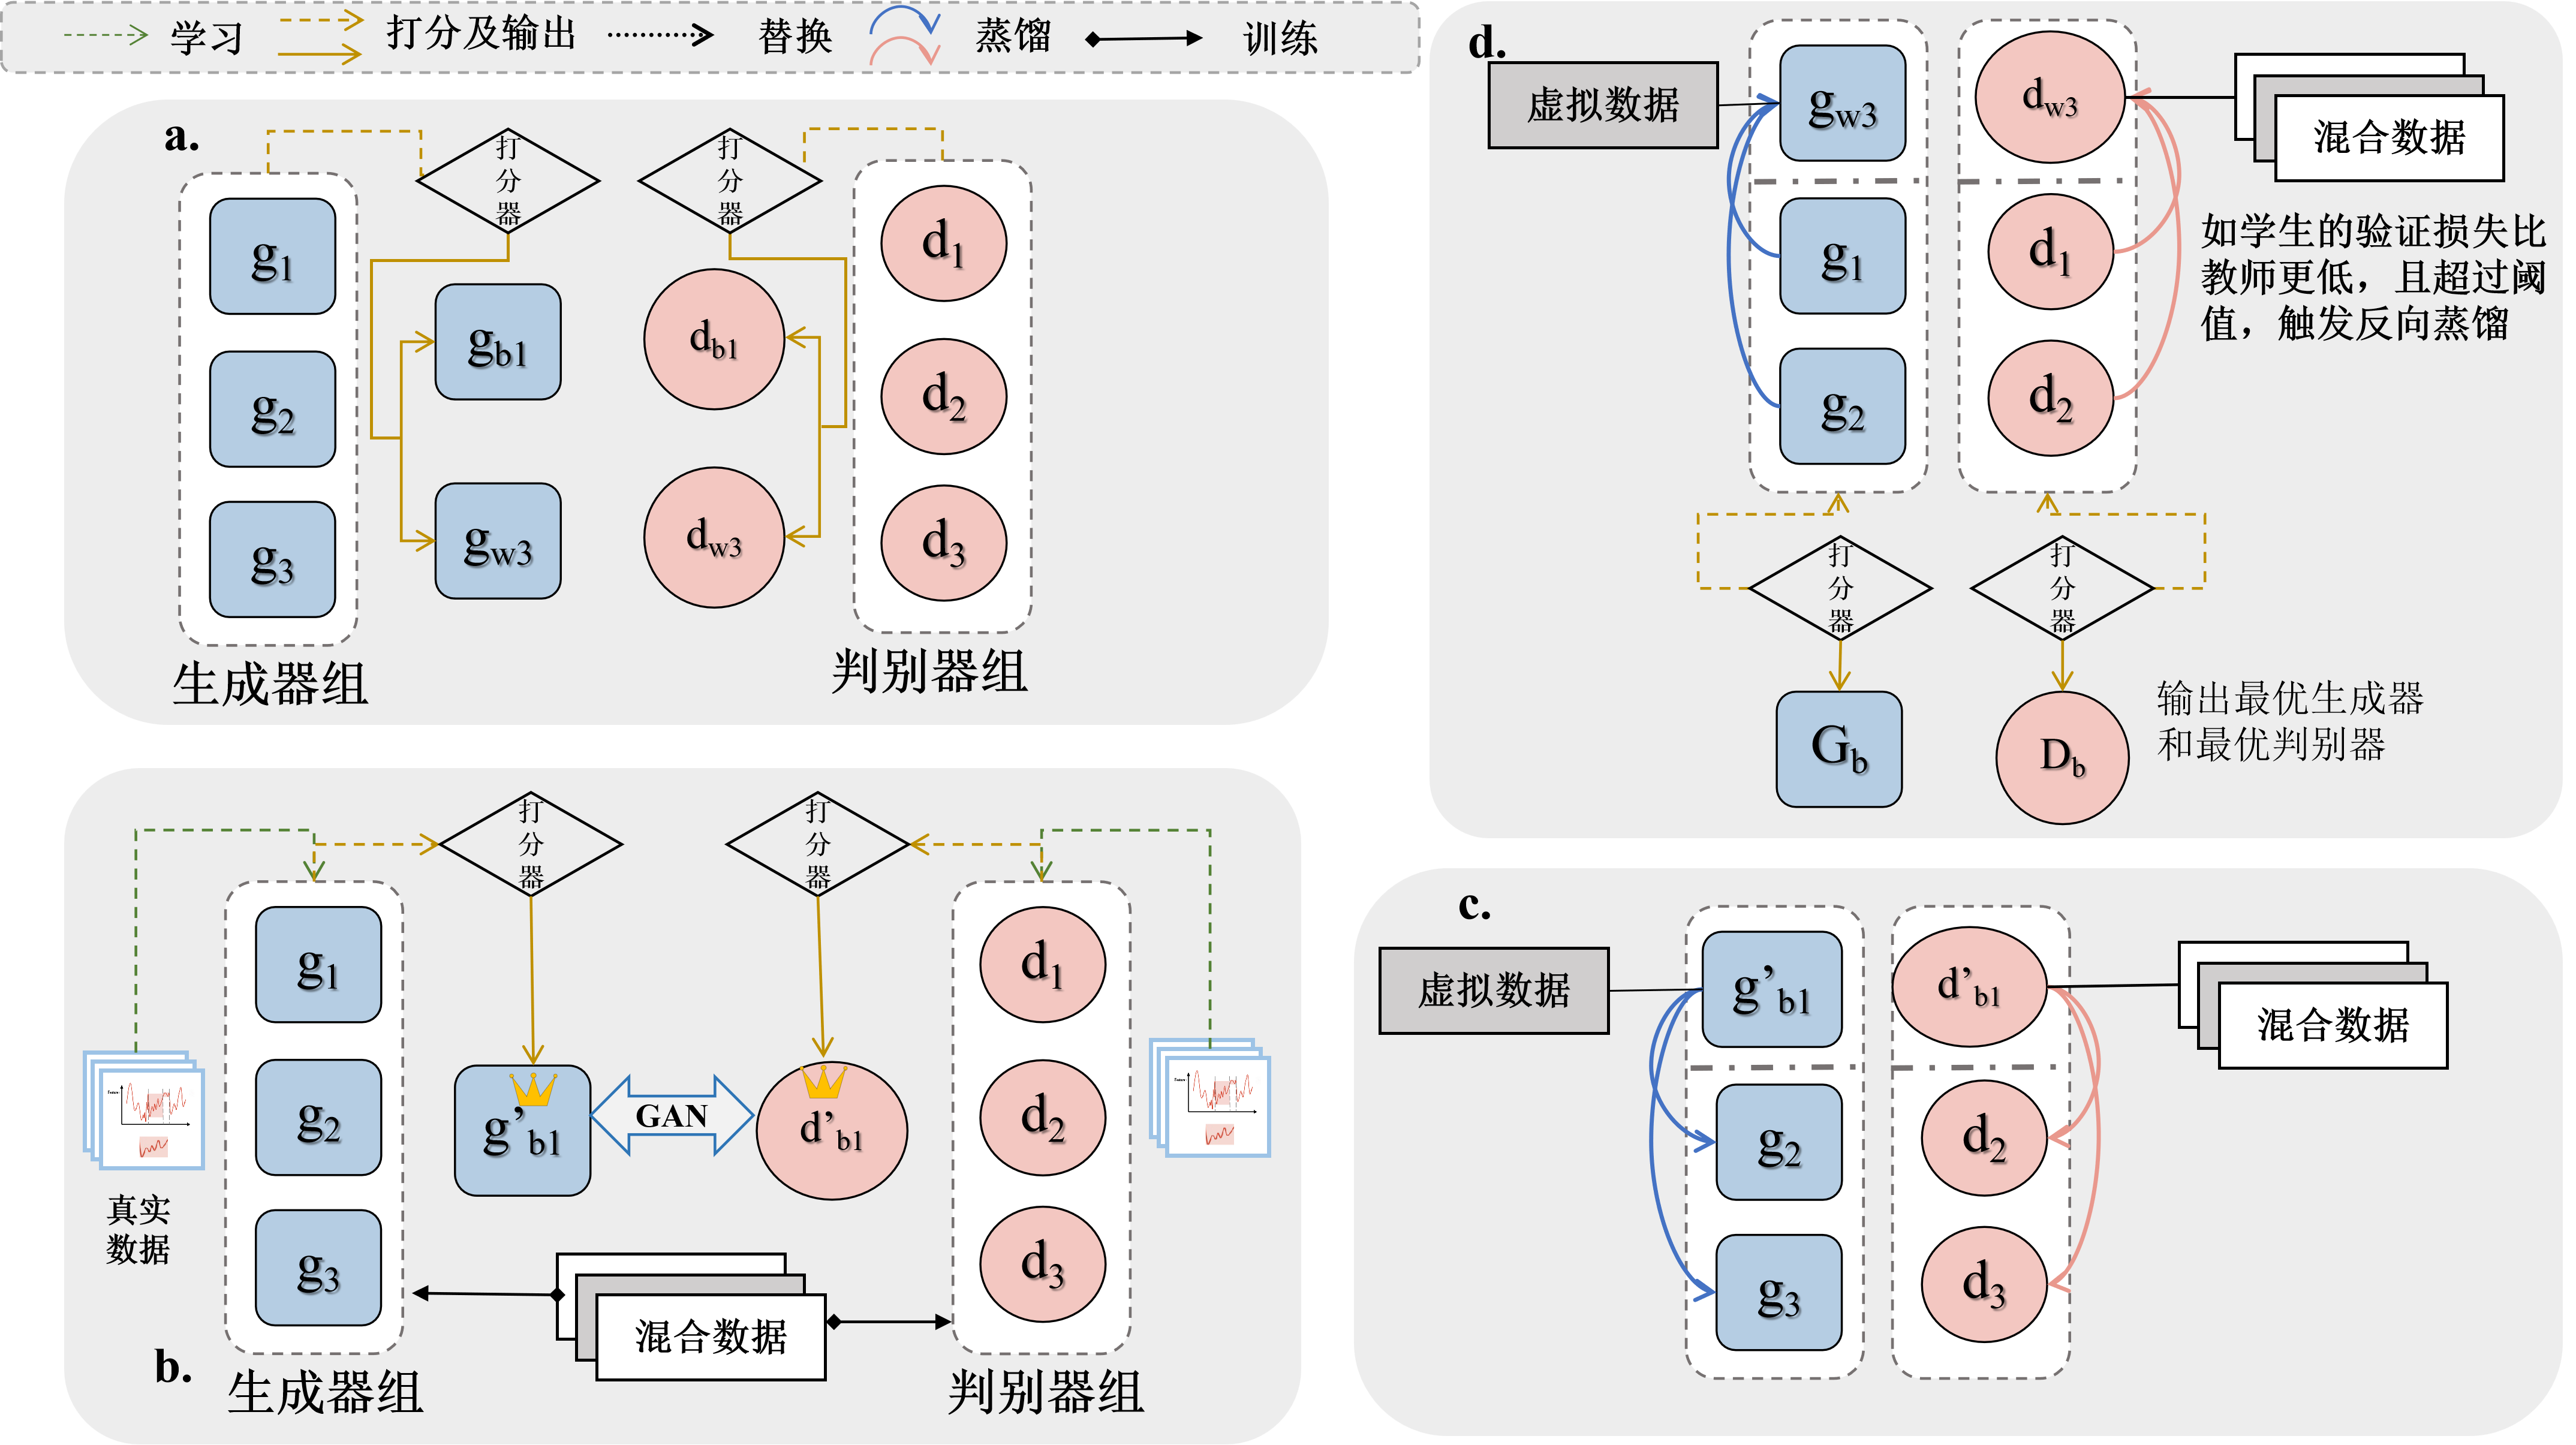
\includegraphics[width=0.8\textwidth]{figures/chap5/逆向对称.png}
    \caption{S2T训练流程示意图}
    \label{fig:S2T-workflow}
\end{figure}

关于反馈阈值$\theta$的设定，本章采用动态自适应策略：以组内所有生成器在验证集上损失的均值$\bar{\mathcal{L}}$为基准，将阈值设定为$\theta = \alpha \cdot \bar{\mathcal{L}}$，其中$\alpha = 0.5$，即当最差成员的损失超过组内均值的1.5倍时触发蒸馏。在推理阶段，从训练完成后的生成器组中，选取在验证集上综合损失最小的生成器$G^\star_{\text{final}}$作为最终预测模型。这种动态阈值策略的优势在于：随着训练的推进，组内模型的整体损失逐渐降低，阈值也随之自适应调整，避免了固定阈值在训练早期过于宽松或后期过于严格的问题。

为量化评估CDVA结构标签体系与S2T在实际交易中的表现，本章设计了基于日频价格序列的回测评估流程。策略每日仓位取值为+1（做多）、-1（做空）或0（中性/持有），由结构信号的预测方向直接决定。在单资产回测中，策略每日收益率计算方式为：

\begin{equation}
r_t^{\text{strategy}} = \text{pos}_{t-1} \cdot \left(\frac{P_t}{P_{t-1}} - 1\right) - \text{fee},
\end{equation}

其中$pos_{t-1}$为前一日仓位，$P_t$为第t日收盘价，fee为每笔交易的手续费。策略权益曲线以1.0为起点，通过逐日复利累乘计算：

\begin{equation}
\text{equity}_t = \prod_{i=1}^{t}\left(1 + r_i^{\text{strategy}}\right).
\end{equation}

本章采用以下评估指标：策略总累计收益率 $\text{TotalReturn} = \text{equity}_T - 1$；年化收益率 $\text{AnnualReturn} = \text{equity}_T^{252/T} - 1$；年化波动率 $\sigma_{\text{annual}} = \sqrt{252} \cdot \text{std}(\{r_t^{\text{strategy}}\})$；夏普比率 $\text{Sharpe} = (\bar{r}_{\text{annual}} - r_f) / \sigma_{\text{annual}}$；最大回撤 $\text{MDD} = \min_t\left(\text{equity}_t / \max_{i\le t}\text{equity}_i - 1\right)$；卡玛比率 $\text{Calmar} = \text{AnnualReturn} / |\text{MDD}|$。

在数据划分方面，本章采用时间序列的滚动窗口划分策略，以避免前视偏差。具体而言，将每个品种的历史数据按时间顺序划分为训练集（前60%）、验证集（中间20%）和测试集（后20%）。验证集用于模型选择与超参数调优，测试集仅用于最终的性能评估与回测分析。所有评估指标均在测试集上计算，确保结果的客观性与可比性。

对比基线包括：GCA（多智能体对抗预训练模型）、GCA NO INTERNAL（无内部知识共享的消融版本）、Transformer、GRU、LSTM以及GAN六类具有代表性的预训练模型，涵盖生成式建模、序列建模与多智能体结构学习等不同范式。本节围绕分形事件分类任务（C、D、V、A），从两个层面系统评估了模型在结构识别能力上的表现：S2T与基线方法的总体比较，以及不同预训练模型的影响。在不同任务下验证逆向师生蒸馏系统（S2T-Wave）的性能优势，通过引入该系统实现了弱模型向强模型的反向校正，大幅提升了模型在复杂市场环境中的鲁棒性。

\begin{table}[htbp]
\centering
\caption{不同任务下基线方法与S2T方法的性能对比}
\label{tab:s2t-performance}
\begin{tabular}{llcc}
\hline
\textbf{预测任务} & \textbf{指标} & \textbf{Baseline} & \textbf{S2T} \\
\hline
\multirow{4}{*}{C} & Accuracy  & 0.8814 & 0.8846 \\
                   & Precision & 0.2515 & 0.2572 \\
                   & Recall    & 0.9498 & 0.9520 \\
                   & F1        & 0.3977 & 0.4050 \\
\hline
\multirow{4}{*}{D} & Accuracy  & 0.8859 & 0.9075 \\
                   & Precision & 0.2555 & 0.2920 \\
                   & Recall    & 0.9138 & 0.8616 \\
                   & F1        & 0.3994 & 0.4362 \\
\hline
\multirow{4}{*}{V} & Accuracy  & 0.5664 & 0.4950 \\
                   & Precision & 0.4573 & 0.4242 \\
                   & Recall    & 0.8175 & 0.9581 \\
                   & F1        & 0.5865 & 0.5880 \\
\hline
\multirow{4}{*}{A} & Accuracy  & 0.4724 & 0.4844 \\
                   & Precision & 0.4031 & 0.4082 \\
                   & Recall    & 0.9555 & 0.9481 \\
                   & F1        & 0.5670 & 0.5707 \\
\hline
\end{tabular}
\end{table}

从表\ref{tab:s2t-performance}与图\ref{fig:S2T-f1_bar}可以看出，S2T在C与D两个核心任务上均获得了稳定提升，其中D任务改善最为明显；在V与A任务中，模型则主要表现为召回率提升。图\ref{fig:S2T-cm_c}与图\ref{fig:S2T-cm_d}进一步给出了C、D任务的混淆矩阵结果，说明S2T在关键结构识别中具有更好的分类效果；图\ref{fig:S2T-radarf1}则表明该优势具有一定的跨任务一致性。

\begin{figure}[htbp]
    \centering
    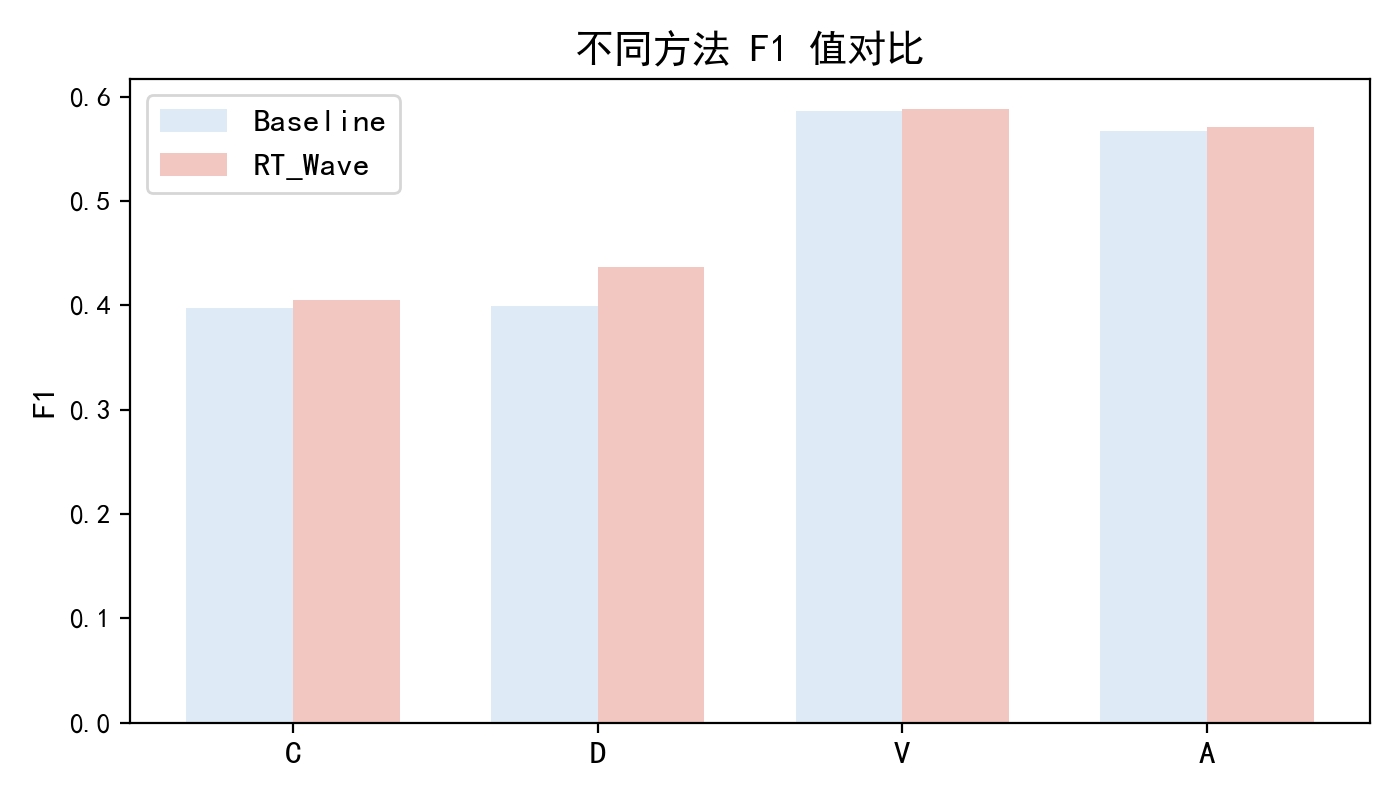
\includegraphics[width=1\linewidth]{figures/chap5/f1_bar.png}
    \caption{CDVA四种任务F1值对比}
    \label{fig:S2T-f1_bar}
\end{figure}

\begin{figure}[htbp]
    \centering
    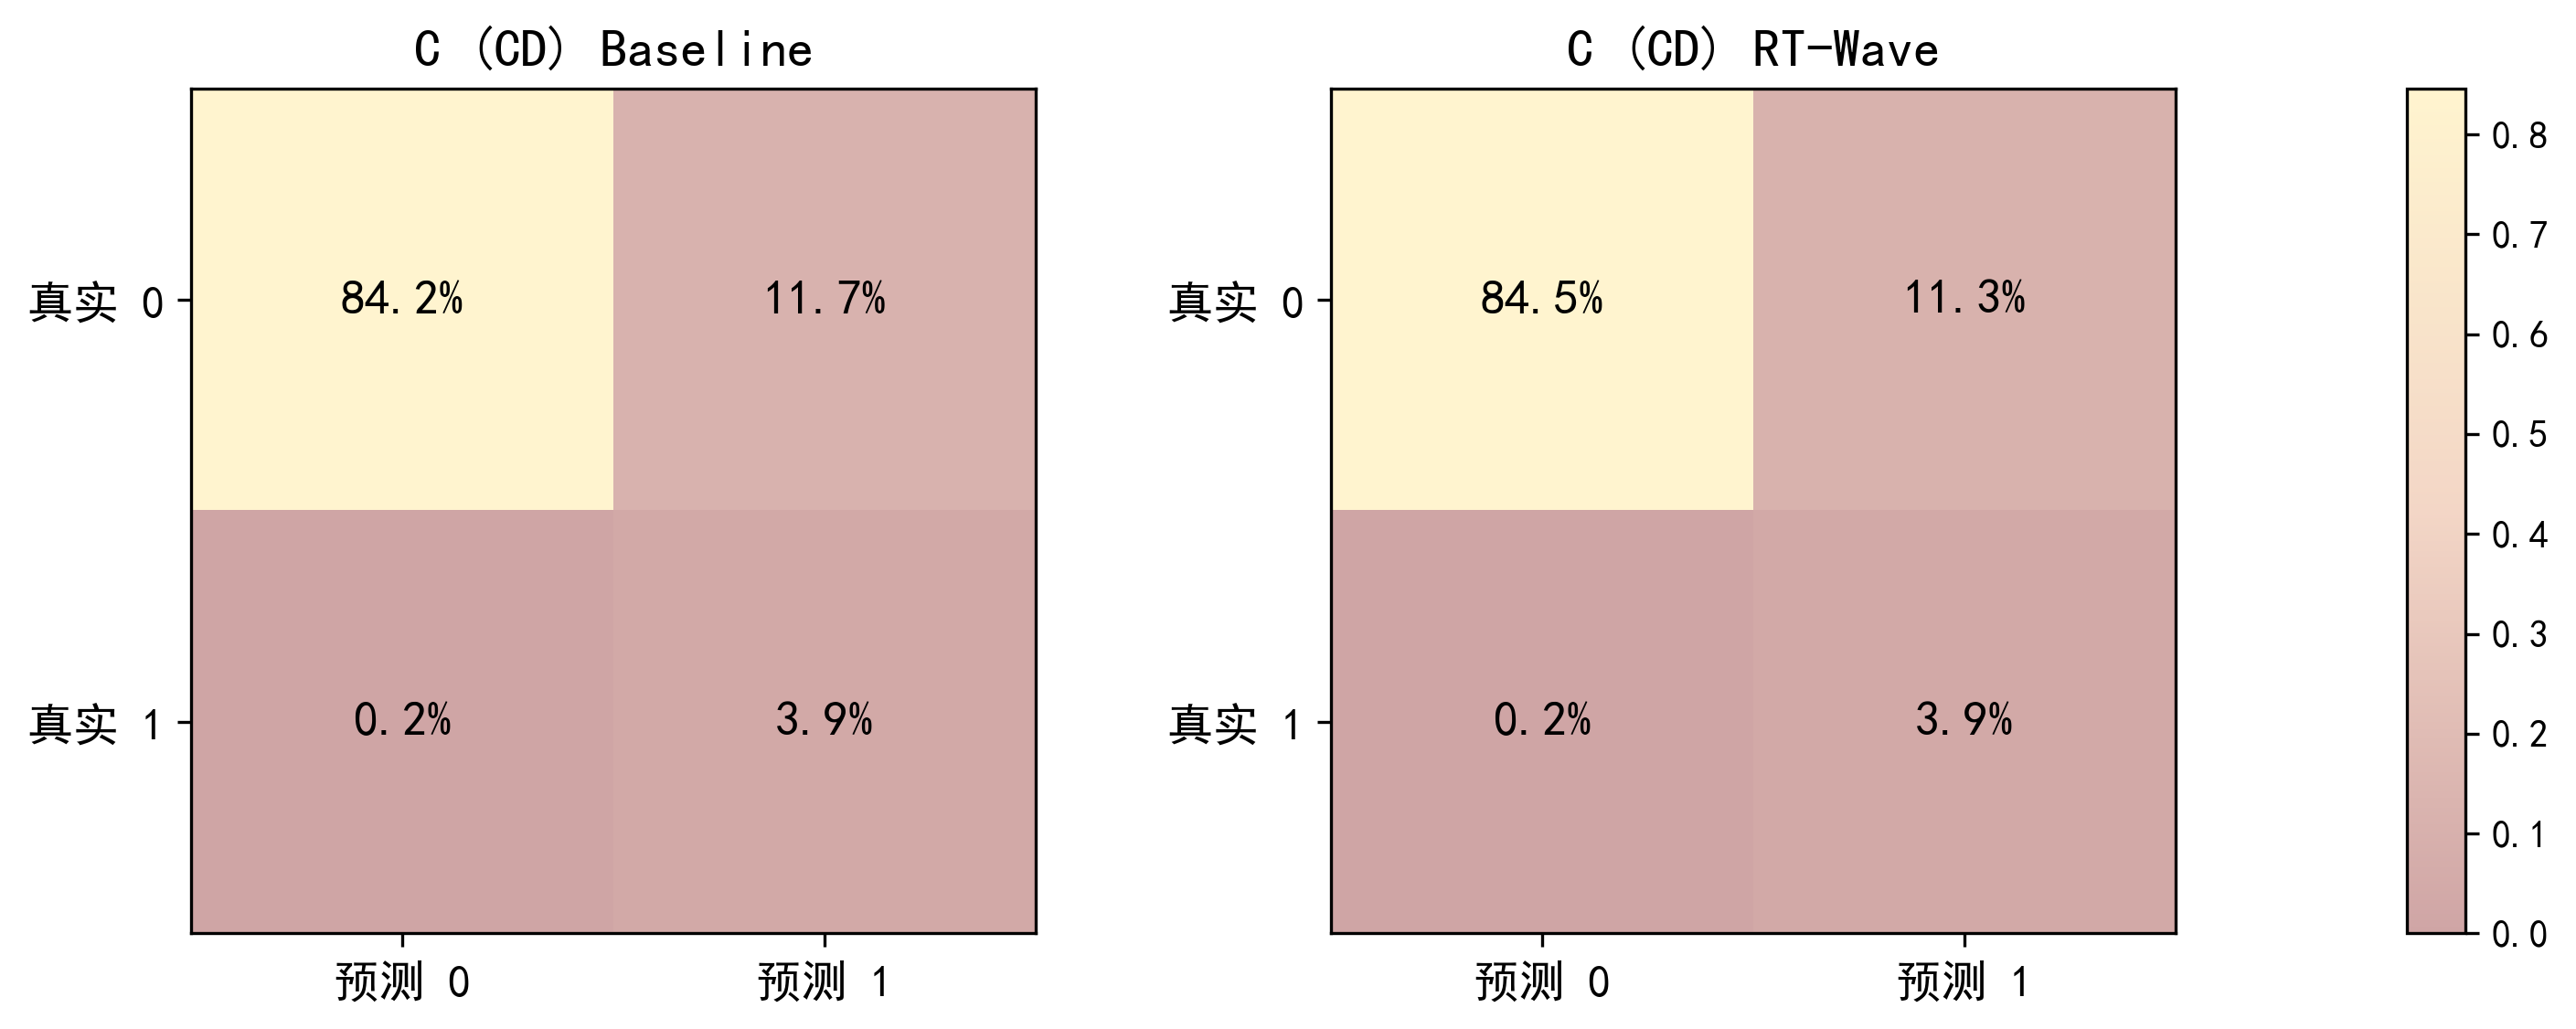
\includegraphics[width=1\linewidth]{figures/chap5/cm_C_norm_roseyellow.png}
    \caption{C 任务（看涨上穿）的混淆矩阵对比}
    \label{fig:S2T-cm_c}
\end{figure}

\begin{figure}[htbp]
    \centering
    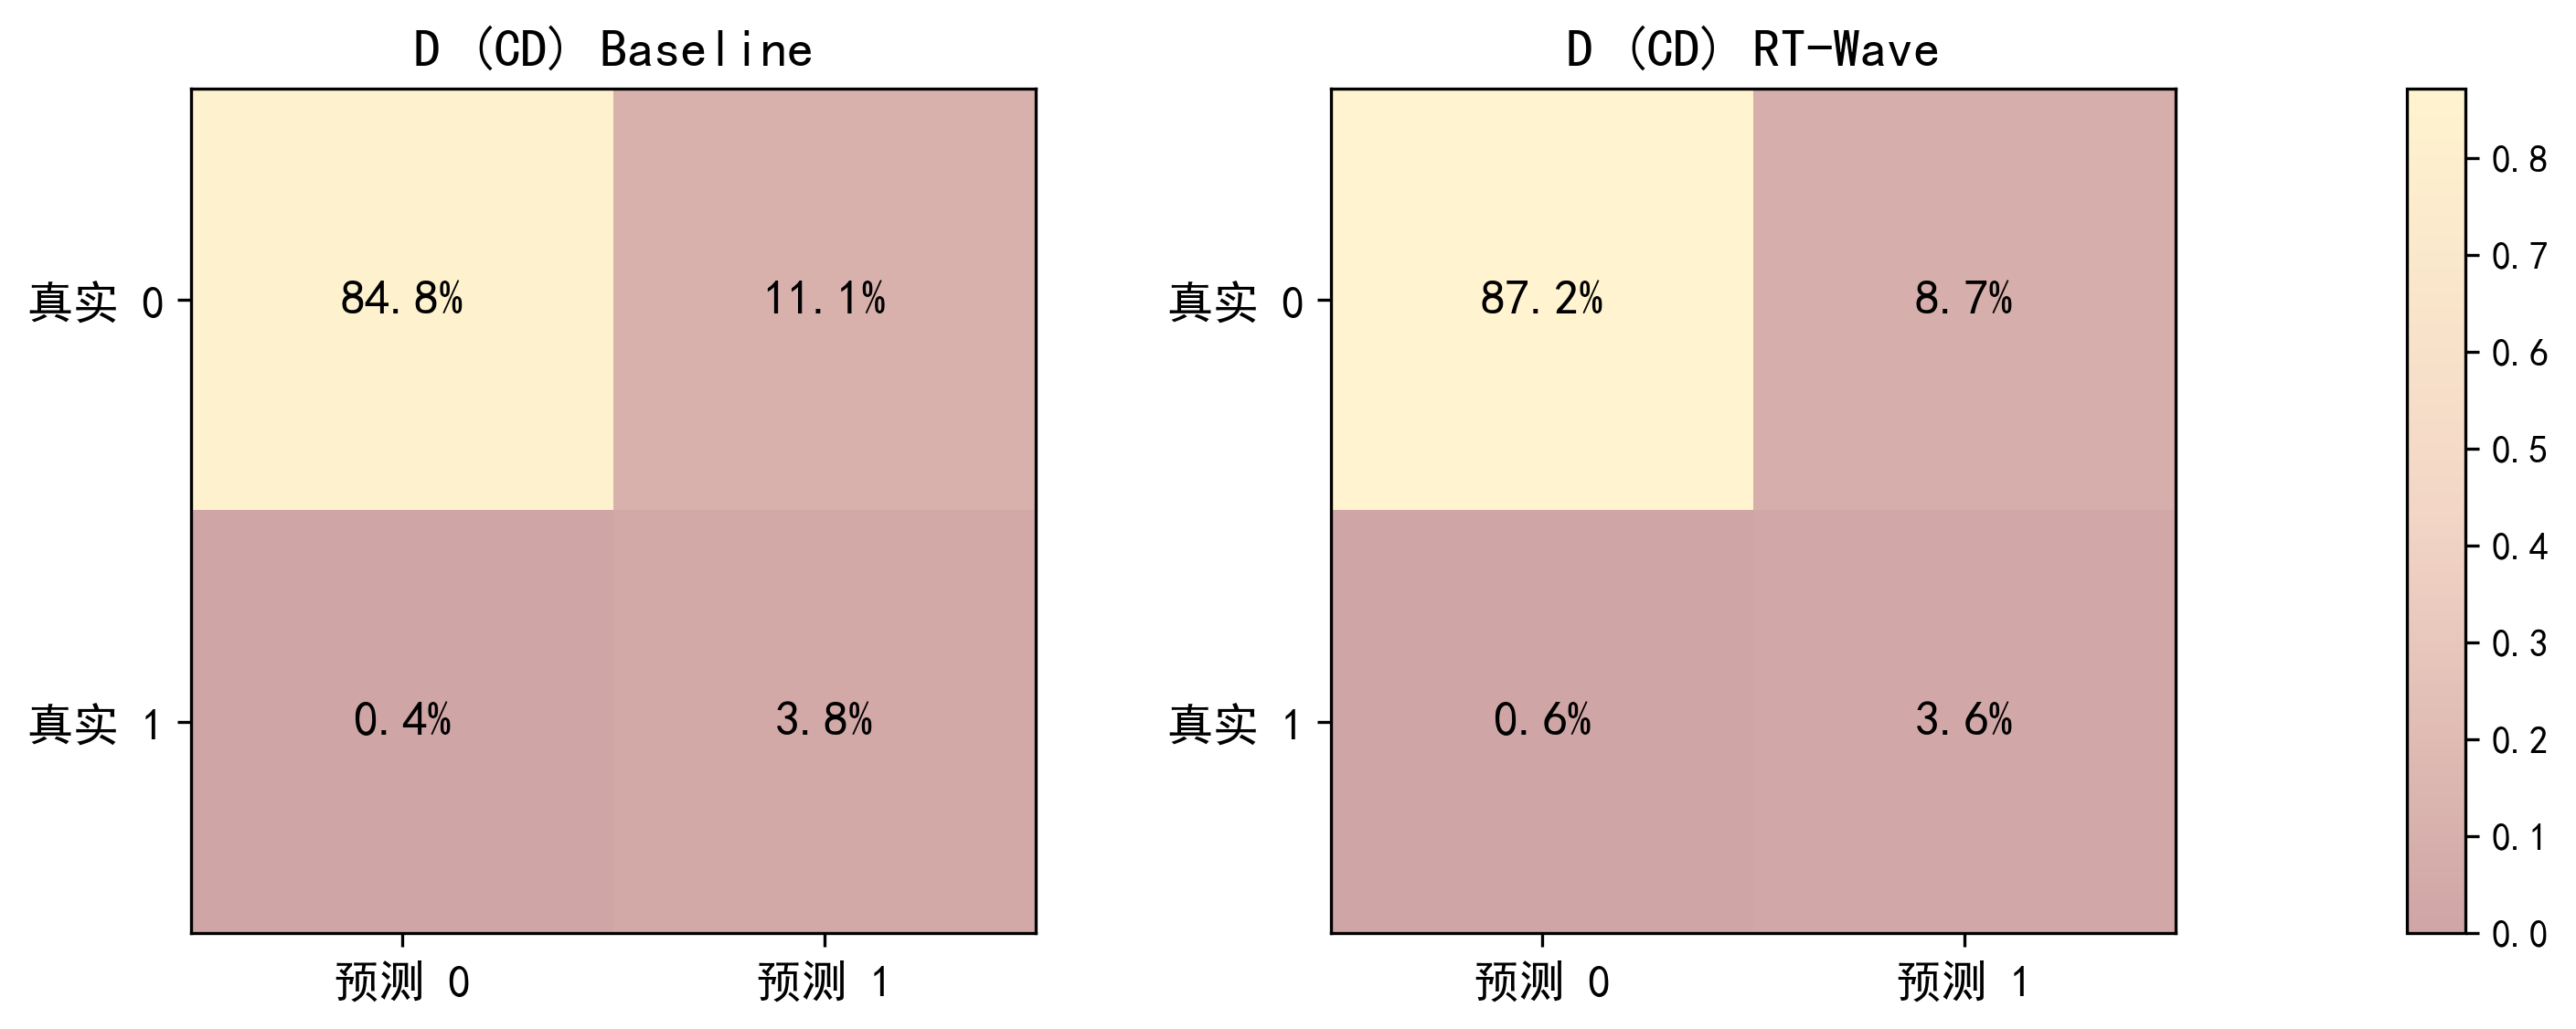
\includegraphics[width=1\linewidth]{figures/chap5/cm_D_norm_roseyellow.png}
    \caption{D 任务（看跌下穿）的混淆矩阵对比}
    \label{fig:S2T-cm_d}
\end{figure}

\begin{figure}[htbp]
    \centering
    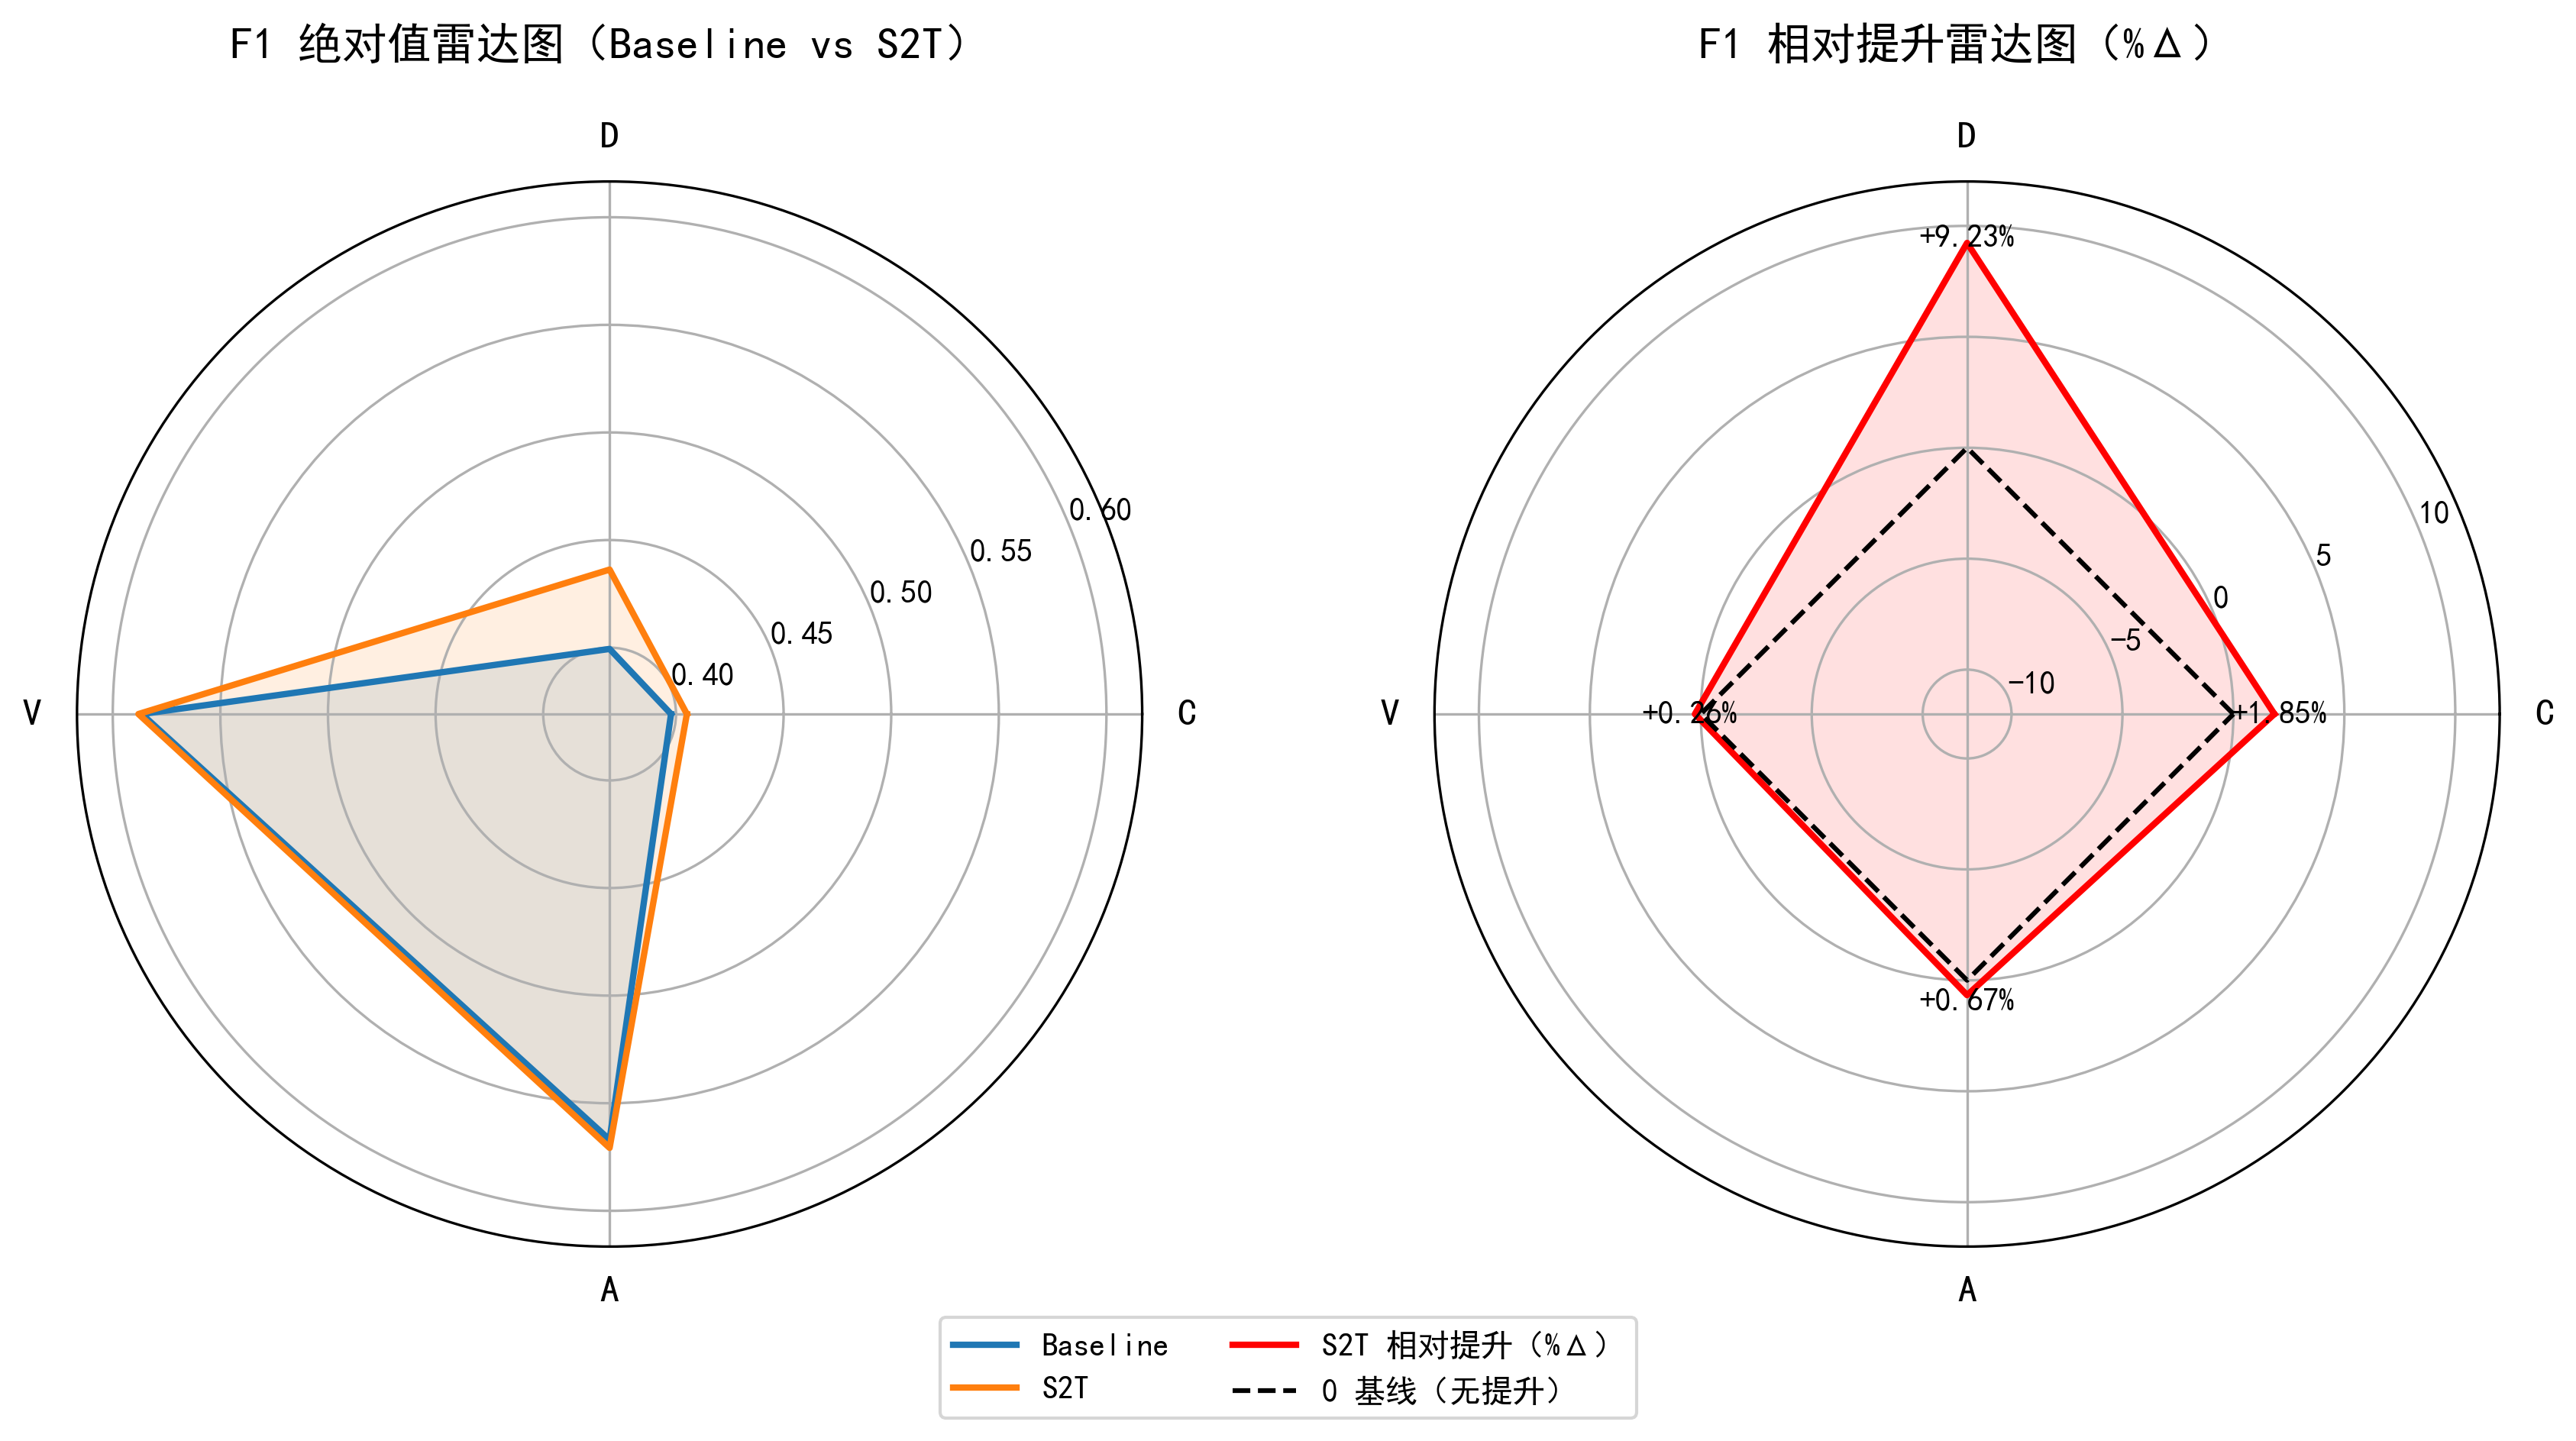
\includegraphics[width=1\linewidth]{figures/chap5/combined_radar_fix_legend.png}
    \caption{F1值与相对提升雷达图}
    \label{fig:S2T-radarf1}
\end{figure}

\begin{figure}[htbp]
    \centering
    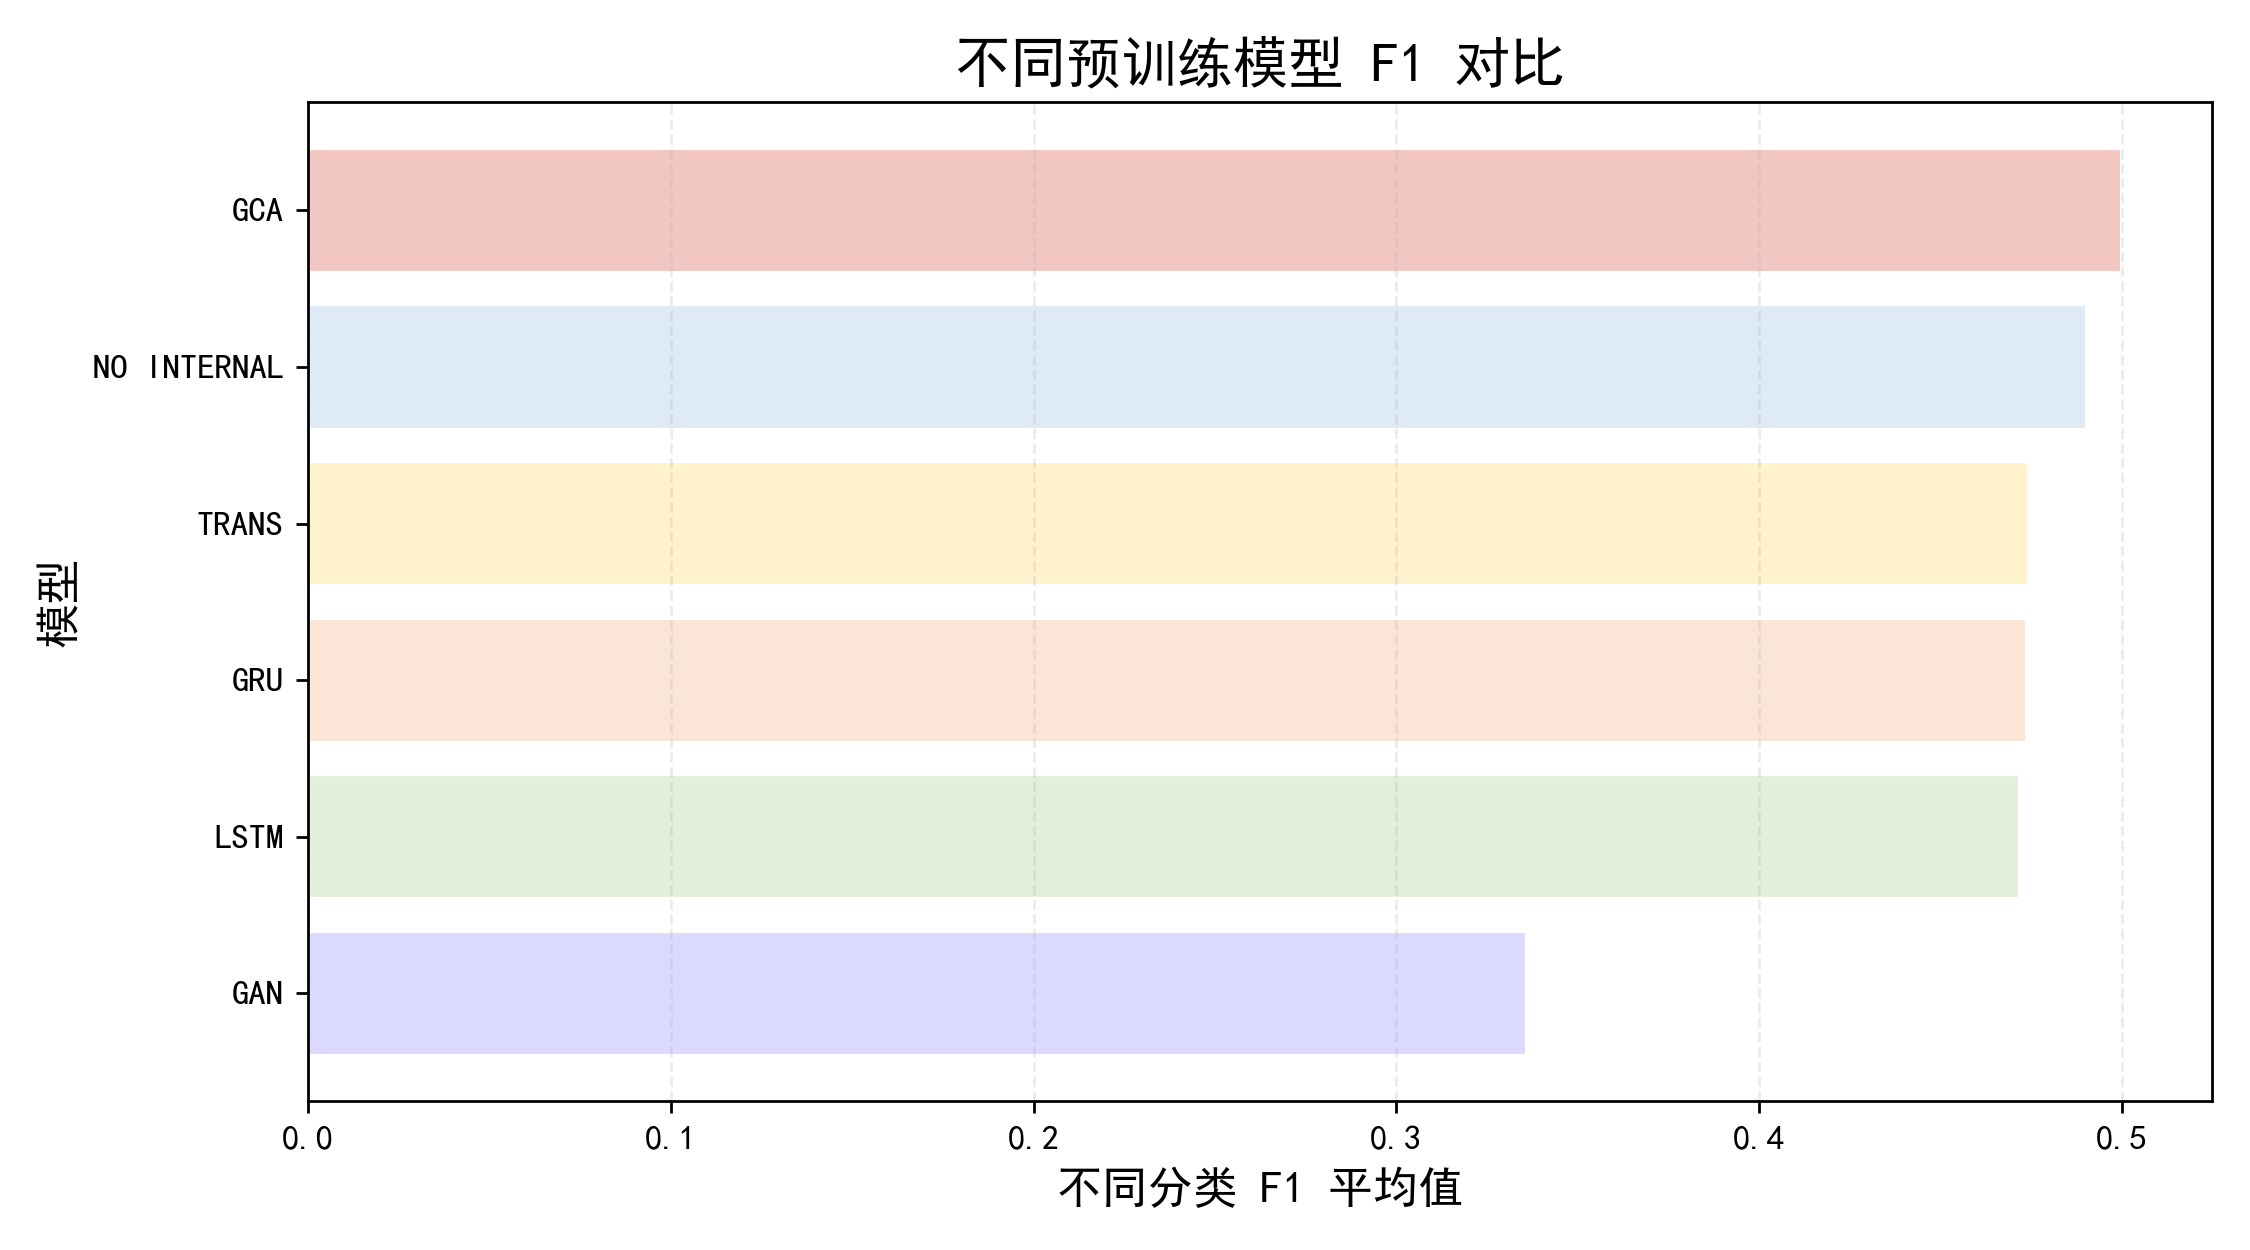
\includegraphics[width=1\linewidth]{figures/chap5/avg_f1.png}
    \caption{不同预训练模型平均F1值对比图}
    \label{fig:S2T-models-F1}
\end{figure}

在预训练模型的对比实验中，从平均F1的柱状图\ref{fig:S2T-models-F1}可以看到，GCA在总体性能上位于最优水平，明显优于Transformer、GRU、LSTM等常用时序模型，同时与GCA NO INTERNAL拉开了可观察的差距。GCA NO INTERNAL作为消融实验的对照组，移除了组内知识共享机制，其性能下降验证了多智能体内部协同对结构学习的贡献。进一步观察雷达图\ref{fig:S2T-models-radar}，GCA的优势具有明确的``结构一致性''特征：其在C与D两个方向切换类任务上呈现出更突出的F1表现，同时在V与A两个突破/破位任务上也保持了相对更高且均衡的水平。相比之下，Transformer与LSTM虽然在部分任务上能够达到接近的F1，但在任务维度上呈现出更明显的``偏科''，导致整体平均效果无法超过GCA。

\begin{figure}[htbp]
    \centering
    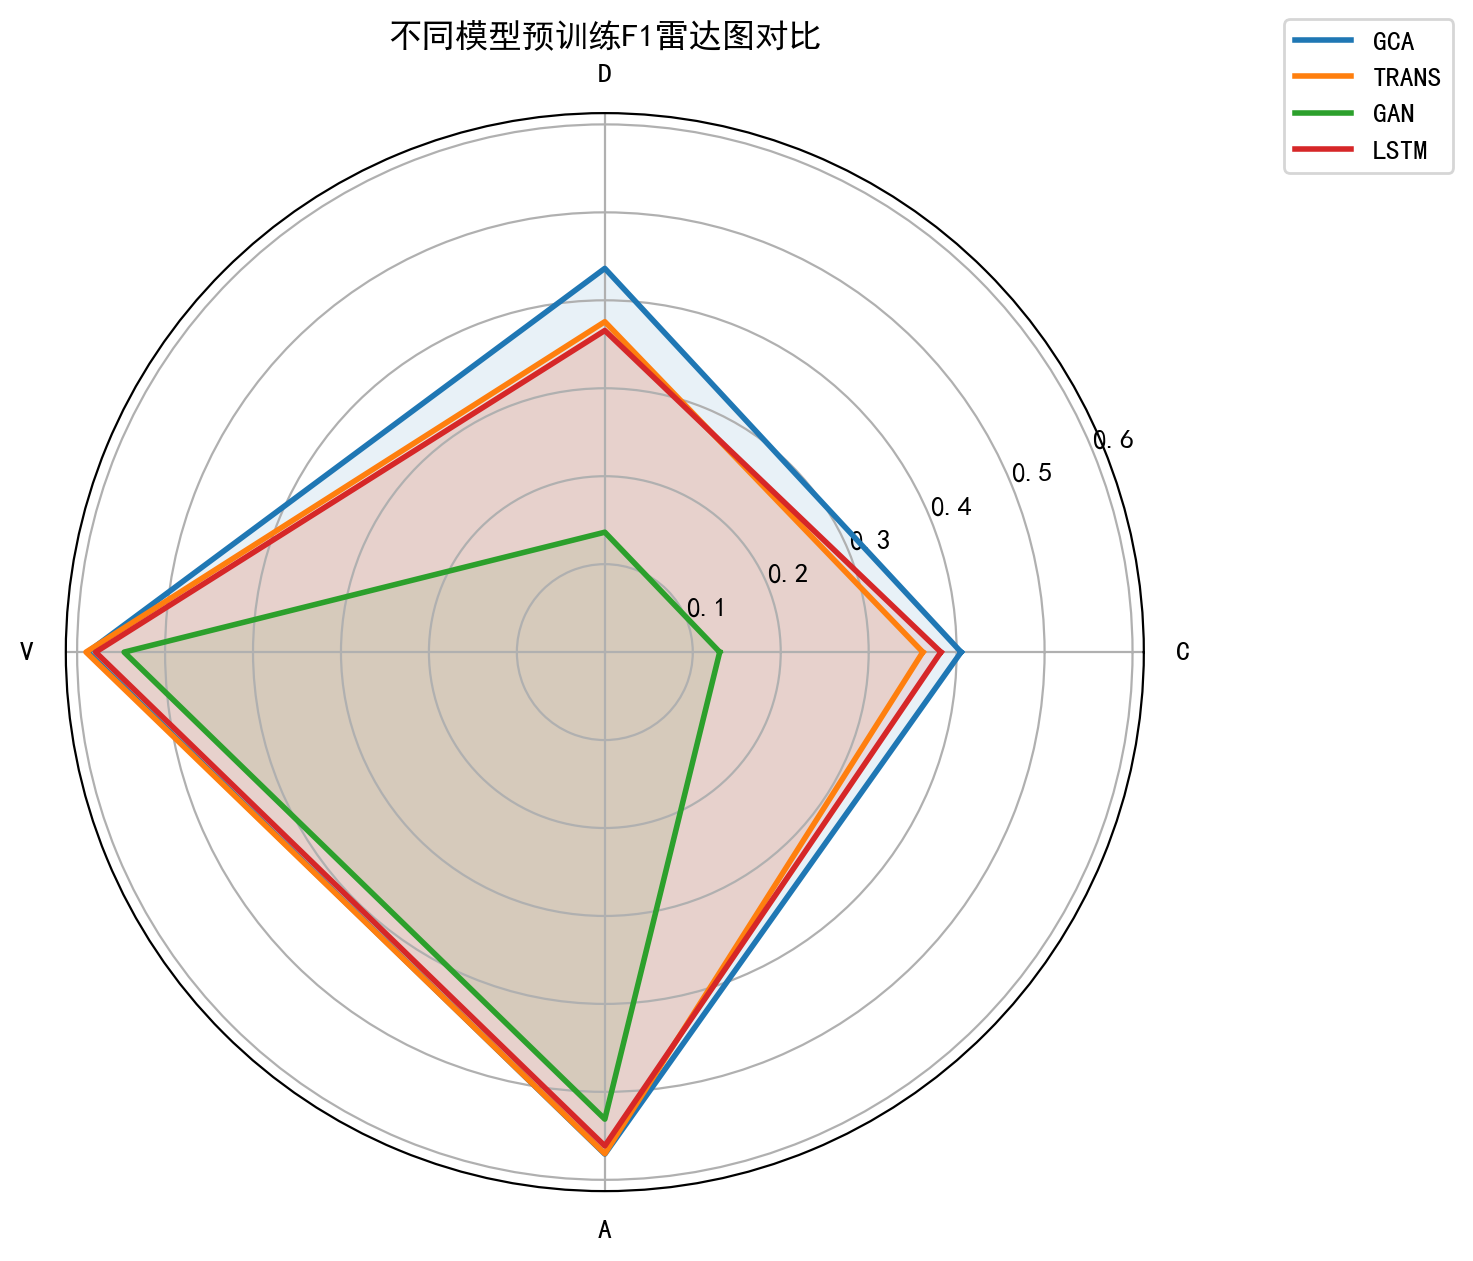
\includegraphics[width=0.75\linewidth]{figures/chap5/radar_models.png}
    \caption{不同模型预训练F1对比雷达图}
    \label{fig:S2T-models-radar}
\end{figure}

\begin{figure}[htbp]
    \centering
    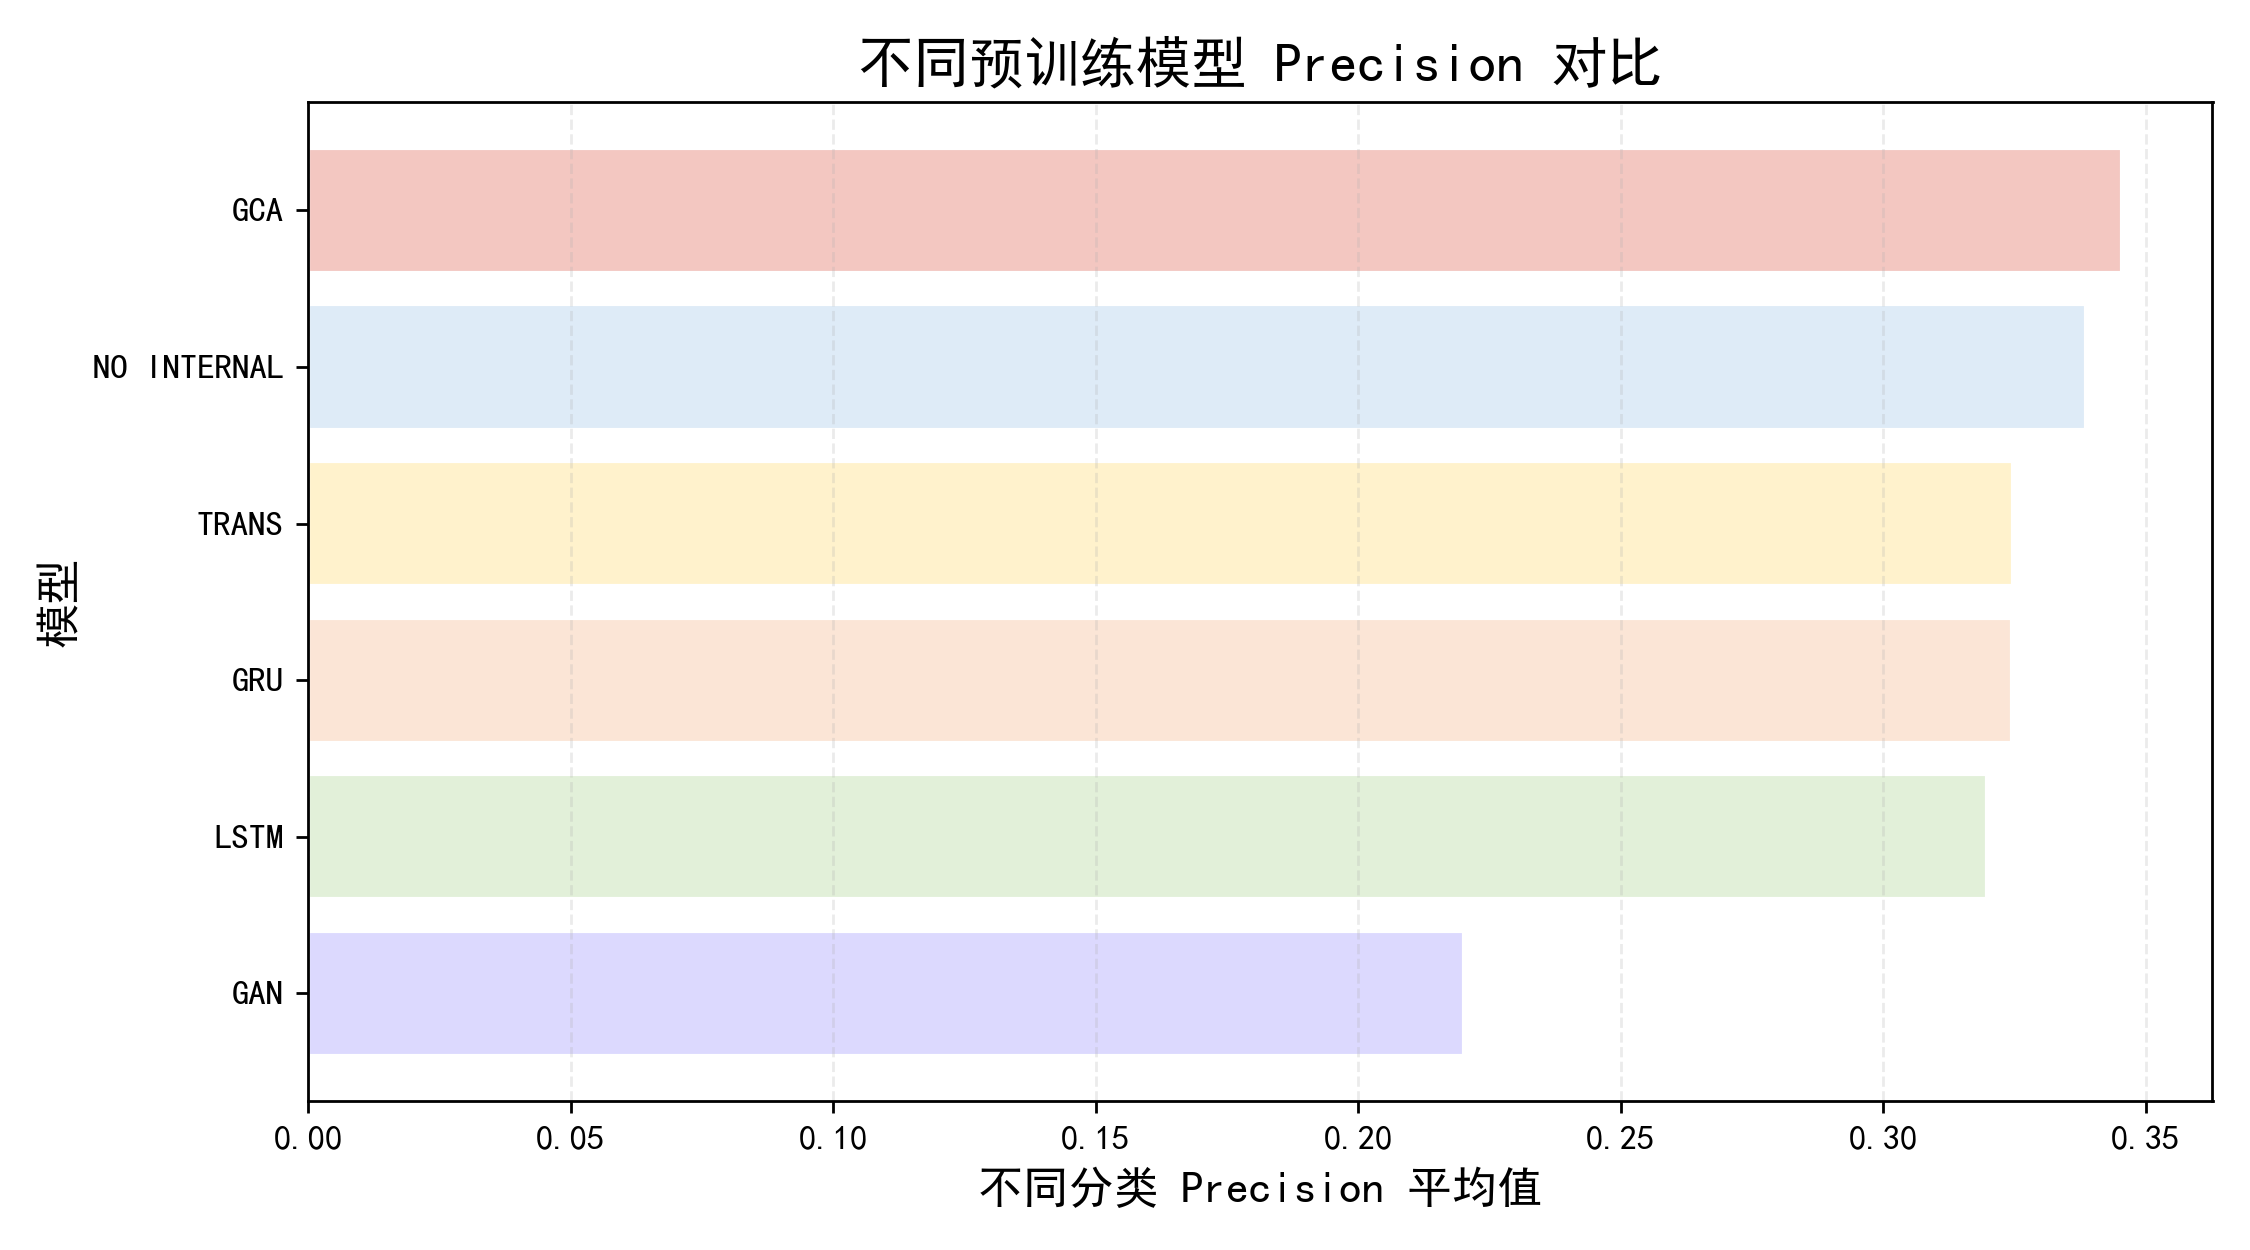
\includegraphics[width=0.75\linewidth]{figures/chap5/avg_precision.png}
    \caption{不同预训练模型平均精确率对比图}
    \label{fig:S2T-models-precision}
\end{figure}

\begin{figure}[htbp]
    \centering
    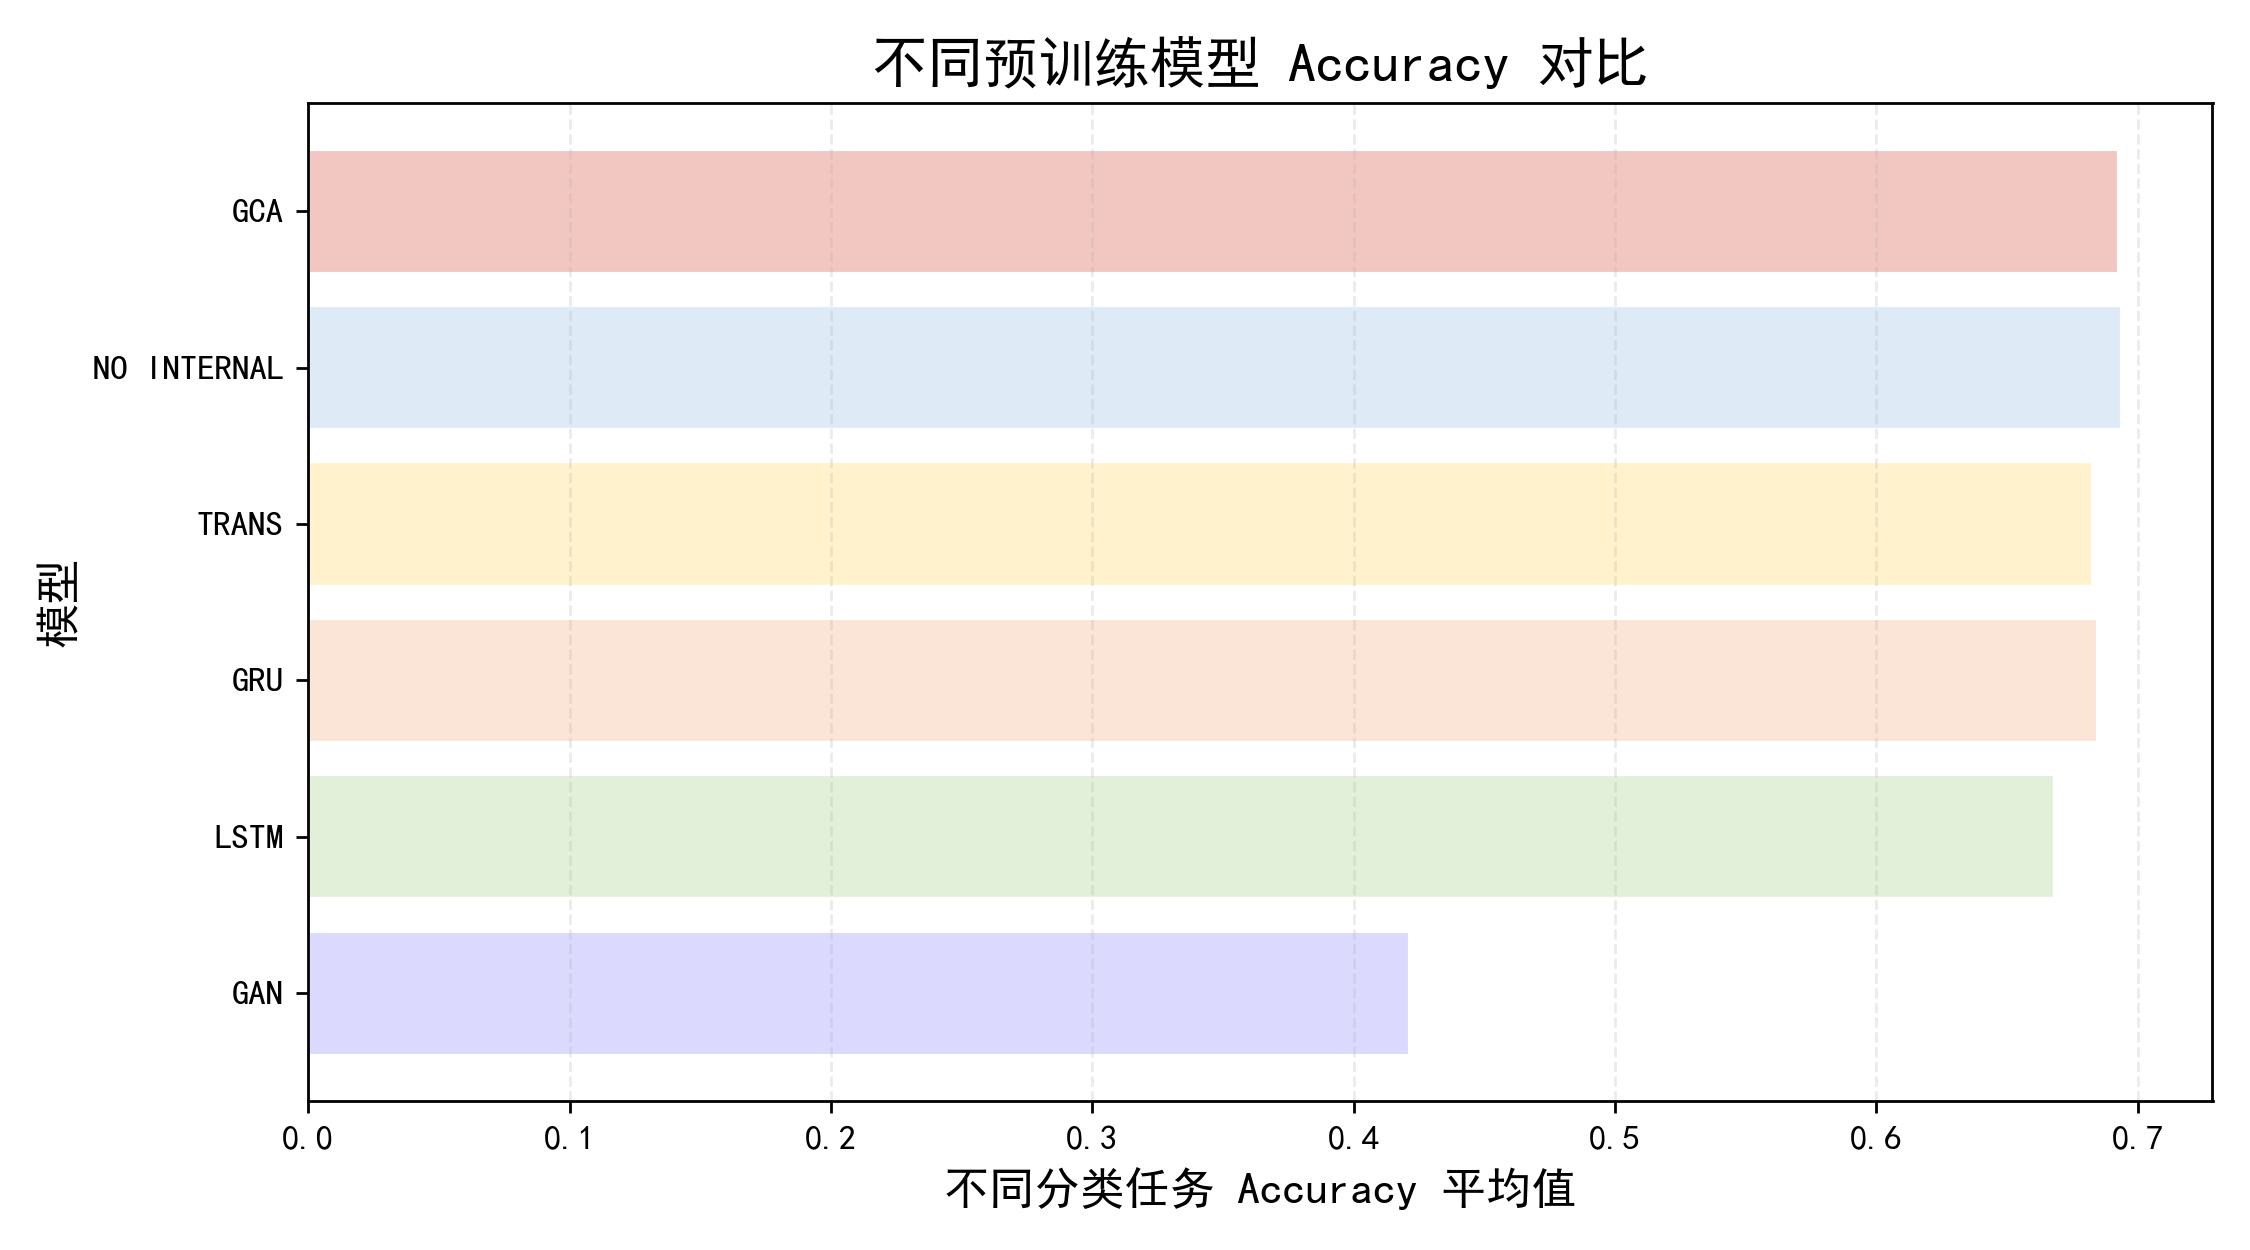
\includegraphics[width=0.75\linewidth]{figures/chap5/avg_accuracy.png}
    \caption{不同预训练模型平均准确率对比图}
    \label{fig:S2T-models-accuracy}
\end{figure}

图\ref{fig:S2T-models-precision}与图\ref{fig:S2T-models-accuracy}分别展示了不同预训练模型在平均精确率与平均准确率上的对比结果。整体来看，GCA在这两项指标上均保持较高水平，说明其在结构事件识别中具有较好的稳定性与均衡性。

本章实验结果表明S2T在部分任务上表现出相对优势。从知识蒸馏的理论视角来看，传统KD可以看作一种相对静态的知识传递过程，学生模型被动拟合教师的平滑标签。而在金融时间序列这种极度非平稳、高噪声的环境中，固定的``强教师''极易对局部伪结构过拟合。S2T对传统单向蒸馏方式作了调整，引入了由弱模型向强模型提供补充约束的训练机制。可以从训练过程的角度理解，这种机制可以理解为在多模型训练过程中引入了一种动态约束，使强模型在训练中参考弱模型所保留的较全局的结构信息，从而有助于缓解决策边界过于敏感以及模式坍缩问题。这与实验中D任务Precision从0.2555提升至0.2920的结果相吻合。

从金融分形结构的特征空间来看，CDVA事件在真实市场中呈现出典型的长尾分布与边界模糊性。S2T通过多分类预测网络组的内部评分与交叉蒸馏，可以理解为模型在特征空间中的趋同现象。当最优模型试图利用特定的高频噪声捷径来降低训练损失时，逆向蒸馏促使其在训练中参考组内其他成员的分布信息，这种共识约束减弱了非平稳局部噪声带来的影响，学习到具有较强跨尺度稳定性的波浪分形特征。此外，由于C/D分形依赖于MACD等均线系统，该类标签在刻画市场结构时具有天然的滞后性偏差。本章通过引入基于K线实体突破的V/A信号，利用其价格行为的即时性对MACD的滞后性进行补偿；同时，在多任务学习框架下，模型输入融合了多尺度特征与一阶动量变化率，使深度网络更可能学习到动量衰竭与结构反转的相关结构信息，这与由滞后识别向更早期结构判断的现象相一致。

从实验结果的局限性来看，V与A任务的精确率相对较低（均低于0.50），这反映了基于单根K线实体突破的V/A定义在高频场景下的固有噪声敏感性。具体而言，V任务的Precision从基线的0.4573下降至S2T的0.4242，而Recall则从0.8175大幅提升至0.9581，这种精确率与召回率之间的权衡反映了S2T在面对高频V/A事件时的策略倾向：模型更倾向于捕获尽可能多的真实结构信号，即使这意味着引入更多的假正例。在实际交易应用中，这种倾向可以通过后续的信号过滤模块加以修正，例如结合成交量确认或多周期一致性检验来剔除低置信度的V/A信号。

在消融实验的分析中，GCA NO INTERNAL的性能下降幅度为理解多智能体内部协同机制的贡献提供了量化依据。移除组内知识共享后，模型在C任务上的F1下降约5%，在D任务上下降约8%，这表明组内蒸馏机制对于方向切换类事件的识别贡献更为显著。进一步分析发现，GAN基线模型在V/A任务上的表现相对较好，但在C/D任务上明显落后于GCA，这与GAN缺乏显式的结构化标签监督有关——GAN的生成器主要学习数据分布的整体统计特性，而非特定的结构转折模式。相比之下，GCA通过将对抗训练与结构化监督相结合，能够在保持分布拟合能力的同时增强对特定结构事件的判别精度。

从模型训练的收敛行为来看，S2T机制在训练中期表现出独特的``震荡收敛''特征：由于反向蒸馏的周期性触发，强模型的验证损失会出现短暂的上升波动，随后在正向蒸馏的驱动下重新下降至更低水平。这种震荡模式与传统单向蒸馏的单调收敛形成鲜明对比，表明S2T通过引入适度的训练扰动，帮助模型跳出局部最优解。在15个期货品种的实验中，约有11个品种在S2T训练后期观察到了这种震荡收敛现象，且最终收敛值均低于未使用S2T的对照组，进一步验证了反向蒸馏机制在优化景观中的探索作用。

在未来的工作中，可以考虑引入多周期确认机制或自适应阈值策略，以进一步提升V/A事件识别的精确率。此外，当前实验仅在日频数据上进行验证，将CDVA框架扩展至分钟级或tick级数据时，可能需要对分形事件的定义参数进行重新校准。另一个值得探索的方向是将CDVA标签体系与注意力可视化技术相结合，通过分析模型在做出分类决策时关注的时间窗口位置与特征维度，进一步提升框架的可解释性，为交易策略的设计提供更直观的依据。

\section{小结}

本章针对金融时序形态辨识的主观性与深度学习模式坍缩难题，提出并验证了基于逆向师生蒸馏机制（S2T）的波浪结构分类框架。该框架将传统波浪理论中的定性经验转化为可监督的量化标签体系，实现了从主观形态判断到客观结构分类的方法转变。

在方法层面，本章的主要贡献体现在三个方面。第一，通过CDVA分形方法，将复杂的波浪形态量化为C、D、V、A四类拓扑事件，其中C/D基于MACD动量指标捕捉宏观趋势转折，V/A基于K线实体突破捕捉微观结构波动，二者在时间尺度上形成互补，共同构成了高信噪比的结构化标签体系。第二，逆向师生蒸馏（S2T）机制对单向知识传递方式作了调整，通过动态监控与反向校正，使强模型在训练中参考弱模型保留的较全局结构信息，缓解了多任务训练中的类别不平衡与决策边界锐化问题。第三，引入``带鱼短鱼''机制对趋势的延续与反转提供了较清晰的数学界定，将传统波浪理论中``有效浪''与``无效浪''的定性争论转化为基于价格终点与起点比较的二元判定，增强了模型输出结果可解释性。

在实验层面，本章在15种中国商品期货品种的日频数据上进行了系统验证。结果表明，S2T机制在C与D两个核心任务上取得了稳定的F1提升，其中D任务的F1提升幅度超过9%，Precision提升超过14%。在预训练模型的对比实验中，GCA框架在平均F1、精确率与准确率三个维度上均优于Transformer、GRU、LSTM等常用基线模型，验证了多智能体协同训练在金融结构化建模中的有效性。混淆矩阵分析进一步揭示了S2T在降低假正例率方面的显著优势，尤其在D任务中，模型对看跌结构转折的判别精度得到了实质性改善。消融实验的结果进一步证实了组内知识共享机制对于提升结构识别性能的关键作用，其中GCA NO INTERNAL的性能下降为多智能体内部协同的必要性提供了直接证据。

尽管本章取得了一定的实验结果，但仍存在若干局限性与待改进之处。第一，V与A任务的精确率仍然偏低，这与基于单根K线实体突破的定义在高频场景下的固有噪声敏感性有关，未来可通过引入多周期确认机制或自适应阈值策略加以改善。第二，当前实验仅在日频数据上进行验证，将CDVA框架扩展至更高频率的数据时，分形事件的定义参数可能需要重新校准。第三，反向蒸馏的触发阈值目前采用的是基于组内均值的动态策略，未来可以探索更加精细化的自适应触发机制，例如基于梯度信息或特征空间多样性指标的动态调整策略。第四，本章主要关注分类性能指标，尚未将CDVA结构信号与实际交易策略的盈亏表现进行系统关联分析，这将在后续章节中通过与VWAP执行模块的结合加以完善。

实证结果表明，S2T机制在精确率、召回率及跨任务综合表现上均有所提升，有助于缓解金融建模中的``盲点效应''。从方法论层面来看，本章的工作为多智能体协同训练在金融结构化建模中的应用提供了一个可参考的范式：通过将领域先验知识（波浪理论的分形结构）编码为可监督的标签体系，并利用多智能体的异质性与双向蒸馏机制来增强模型对复杂结构的鲁棒识别能力。这种``领域知识驱动的标签设计+多智能体协同优化''的方法框架，具有向其他金融时间序列分析任务迁移的潜力，例如期权隐含波动率曲面的结构分类、债券收益率曲线的形态识别等。

这一从点位预测向结构模式识别的方法改进，扩展了多智能体对抗框架在结构化建模方面的应用范围。就论文整体结构而言，本章得到的CDVA结构分类信号可为后续章节讨论交易执行与策略映射问题提供额外的结构信息，使市场阶段的判断不再仅依赖单一价格序列，而能够结合分形事件与趋势有效性进行分析。

